\documentclass[10pt, a4paper,english,spanish]{article}
\usepackage[spanish]{babel}
\parindent = 0 pt
\parskip = 11 pt
\usepackage[width=15.5cm, left=3cm, top=2.5cm, height= 24.5cm]{geometry}

\usepackage{amsmath}
\usepackage{amsfonts}
\usepackage{amssymb}
\usepackage[utf8]{inputenc}
\usepackage{graphicx}
\usepackage{verbatim}
\usepackage{color}
\usepackage{amsmath}
\usepackage{graphicx}
\usepackage[colorinlistoftodos]{todonotes}
\usepackage{multicol}
\usepackage{makeidx}
\usepackage{hyperref}
\usepackage{caption}
\usepackage{amsfonts}
\usepackage{amssymb}
\usepackage{amsmath}
\usepackage[utf8]{inputenc}
\usepackage{verbatim}
\usepackage{listings}
\usepackage{algpseudocode}
\usepackage{courier}
\usepackage{enumitem}
\usepackage{placeins}
\usepackage{booktabs}
% \usepackage[margin=1in]{geometry}


\newcommand{\BigO}[1]{\ensuremath{\operatorname{O}\bigl(#1\bigr)}}
\newtheorem{proposition}{Proposici\'on}
\lstset{language=C++, showstringspaces=false, tabsize=2, breaklines=true, title=\lstname}

\makeindex

\begin{document}
\newgeometry{margin=2cm}
\pagenumbering{gobble}
\raggedleft

\includegraphics[width=8cm]{caratula/logo1.jpg}\\

\raggedright
\vspace{3cm}
{\Huge \bfseries Trabajo Práctico 1 \\ Cálculo de isotermas en sectores circulares}
\rule{\textwidth}{0.02in}
\large Jueves 3 de septiembre de 2015 \hfill Métodos Numéricos
\vspace{1.5cm}

\normalsize
\begin{tabular}{|l@{\hspace{5ex}}c@{\hspace{5ex}}l|}
        \hline
        \rule{0pt}{1.2em}Integrante & LU & Correo electrónico\\[0.2em]
        \hline
        \rule{0pt}{1.2em} Nahuel Lascano  & 476/11 &\tt laski.nahuel@gmail.com\\[0.2em]
        \rule{0pt}{1.2em} XXXX & XXXX &\tt XXXX\\[0.2em]
        \rule{0pt}{1.2em} XXXX & XXXX &\tt XXXX\\[0.2em]
        \hline
\end{tabular}

\medskip
En este trabajo aplicamos dos métodos de resolución de sistemas de ecuaciones lineales (factorización LU y eliminación gaussiana) para el cálculo de isotermas de sectores circulares, dadas las temperaturas de las circunferencias interior y exterior. % TODO: agregar algo breve con conclusiones

\medskip
Palabras clave: factorización LU, eliminación gaussiana, sistemas de ecuaciones lineales, matriz banda

\raggedright

\begin{multicols}{2}

\includegraphics[width=8cm]{caratula/logo-uba.png}

\columnbreak
\vspace*{4.5cm}
\raggedleft
\textbf{Facultad de Ciencias Exactas y Naturales}\\
Universidad de Buenos Aires\\
\small
Ciudad Universitaria - (Pabellon I/Planta Baja)\\
Intendente G\"uiraldes 2160 - C1428EGA\\
Ciudad Autonoma de Buenos Aires - Rep. Argentina\\
Tel/Fax: (54 11) 4576-3359\\
http://www.fcen.uba.ar
\end{multicols}

\restoregeometry

\clearpage

\pagenumbering{arabic}

\tableofcontents

\vspace{3cm}

\clearpage

\setlength{\parindent}{10pt}

\section{Introducción teórica}
En el presente trabajo se intenta evaluar computacionalmente la seguridad térmica de un horno circular. El problema presentado consiste en estimar el riesgo que corre el mismo de fracturarse por efecto de la elevada temperatura. Dicho de otro modo, dadas las temperaturas de las paredes internas y externas del horno (obtenidas a través de sensores) se quiere estimar la ubicación de la isoterma de 500$^{o}$C, cuya cercanía a la pared externa es un indicador de la peligrosidad de la estructura.

Dado un corte transversal del horno podemos definir $r_i$ y $r_e$ como los radios de la pared interna y externa, ambos circualres. Nos interesa analizar la temperatura de los puntos entre ellas. Para referirnos a los puntos de dicha corona circular utilizaremos coordenadas polares, por lo que cada punto $P$ quedará definido por un radio $r$ y un ángulo $\theta$. Si llamamos $T(r,\theta)$ a la temperatura del punto $P_{r, \theta}$, podemos utilizar la ecuación del calor de Laplace para encontrar el estado de equilibrio del sistema:

\begin{equation}\label{calor-continuo}
\frac{\partial^2T(r,\theta)}{\partial r^2}+\frac{1}{r}\frac{\partial T(r,\theta)}{\partial r}+\frac{1}{r^2}\frac{\partial^2T(r,\theta)}{\partial \theta^2} = 0 
\end{equation}

la cual debe cumplirse para todos los puntos internos del horno.

Para aproximar dicha ecuación usando sistemas lineales, usamos una discretización de los puntos que nos interesa analizar (todos los pertenecientes a la pared del horno, que forman una corona circular) y discretizamos asimismo la ecuación \ref{calor-continuo}. De esa manera arribamos a un sistema de ecuaciones lineales que podemos representar en su versión matricial como $Ax=b$ y que intentaremos resolver usando dos métodos: la Eliminación Gaussiana y Factorización LU.

Nos interesa comparar estos dos métodos por el tiempo que les lleva resolver un único sistema $Ax=b$ en función de la granularidad de la discretización. Posteriormente podemos complejizar el problema suponiendo que tenemos múltiples mediciones para las temperaturas de las paredes (a lo largo del tiempo), por lo que debemos comparar su performance a la hora de resolver mútiples sistemas $Ax=b_i$ con diferentes vectores $b_i$.

La solución del sistema de ecuaciones nos permitirá conocer el valor de la funcion $T$ en los puntos de la discretización elegida, pero es posible que ninguno de ellos coincida con el valor de la isoterma buscada. Otro objetivo del trabajo será evaluar diferentes formas de estimar esa isoterma y compararlas variando la granularidad de la discretización.


\clearpage

\section{Desarrollo}
% TODO

% Deben  explicarse  los  metodos  numericos  que  utilizaron  y  su  aplicacion  al  problema
% concreto  involucrado  en  el  trabajo  practico.   Se  deben  mencionar  los  pasos  que  si-
% guieron para implementar los algoritmos, las dicultades que fueron encontrando y la
% descripcion de como las fueron resolviendo.  Explicar tambien como fueron planteadas
% y realizadas las mediciones experimentales.  Los ensayos fallidos, hipotesis y conjeturas
% equivocadas,  experimentos  y  metodos  malogrados  deben  gurar  en  esta  seccion,  con
% una breve explicacion de los motivos de estas fallas (en caso de ser conocidas).

\subsection{Armado del sistema de ecuaciones}
De la discretización de la ecuación del calor provista por el informe resulta una nueva ecuación que nos va a servir para armar nuestro sistema discreto:

\begin{equation}\label{calor}
\frac{t_{j-1,k}-2t_{jk}+t_{j+1,k}}{(\Delta r)^2}+\frac{1}{r}\frac{t_{j,k}-t_{j-1,k}}{\Delta r}+\frac{1}{r^2}\frac{t_{j,k-1}-2t_{jk}+t_{j,k+1}}{(\Delta \theta)^2} = 0 
\end{equation}

Esta ecuación vale para cada punto del modelo salvo los límites, sobre los cuales hablaremos en breve.

Para poder armar el sistema $Ax=b$ equivalente, es necesario:
\begin{itemize}
 \item
    Extraer los factores que multiplican a cada una de las cinco incógnitas: $t_{j-1,k}$; $t_{j,k}$; $t_{j+1,k}$; $t_{j,k-1}$ y $t_{j,k+1}$.

    Estos se obtienen de la ecuación \ref{calor}.
    \begin{align*}
        t_{j-1, k}&*(\frac{1}{(\Delta r)^2} - \frac{1}{r_j \Delta r}) \\
        t_{j, k}  &*(\frac{-2}{(\Delta r)^2} + \frac{1}{r_j \Delta r} - \frac{2}{{r_j}^2 (\Delta r)^2}) \\
        t_{j+1, k}&*(\frac{1}{(\Delta r)^2}) \\
        t_{j, k-1}&*(\frac{1}{{r_j}^2(\Delta \theta)^2}) \\
        t_{j, k+1}&*(\frac{1}{{r_j}^2(\Delta \theta)^2})
    \end{align*}
    Por cuestiones de espacio, en adelante llamaremos $M_{j,k}$ al factor que multiplica a la incógnita $t_{j,k}$, $M_{j-1,k}$ al que multiplica a $t_{j-1,k}$ y así sucesivamente. Y resumiremos $Mt_{j,k} = M_{j,k}*t_{j,k}$, $Mt_{j-1,k}=M_{j-1,k}*t_{j-1,k}$.
 \item
    Analizar los ``casos borde'': aquellos puntos donde la ecuación \ref{calor} no vale.
    
    Para evitar confusiones de variables, tomaremos $\theta_0 = 0$ como el menor valor posible de $\theta$ y $\theta_{n-1}$ como el mayor, pues vale $(r_j, \theta_n) = (r_j, \theta_0)$ para cualquier $j$. 
    
    Los casos interesantes para valores de $j, k$ entonces son:
    \begin{enumerate}
     \item La pared interior del horno ($j = 0$; $k = 0, ..., n-1$). La ecuación en esos casos es $t_{0, k} = T_i(\theta_k)$.
     \item La pared exterior del horno ($j = m$; $k = 0, ..., n-1$). La ecuación en esos casos es $t_{m, k} = T_e(\theta_k)$.
     \item El valor mínimo de $\theta$ ($j = 0, ..., m$; $k = 0$). Se debe reemplazar $t_{j, k-1}$ por $t_{j, n-1}$ en todas las ecuaciones correspondientes.
     \item El valor máximo de $\theta$ ($j = 0, ..., m$; $k = n-1$). Se debe reemplazar $t_{j, k+1}$ por $t_{j, 0}$ en todas las ecuaciones correspondientes.
    \end{enumerate}
    Estos últimos reemplazos se pueden resumir en $$(j, k) \Rightarrow (j, k \text{ mod } n)$$
 \item
    Combinar los puntos anteriores para plantear el sistema de ecuaciones a resolver:
    \begin{align*}\label{sistema}
    &t_{0, k} = T_i(\theta_k)                                           &\forall k = 0, ..., n-1  \\
    &t_{m, k} = T_e(\theta_k)                                           &\forall k = 0, ..., n-1  \\
    &Mt_{j-1,k} + Mt_{j,k} + Mt_{j+1,k} + Mt_{j,k-1} + Mt_{j,k+1} = 0  &\forall j=1, ..., m-1; k = 1, ... , n-2 \\
    &Mt_{j-1,0} + Mt_{j,0} + Mt_{j+1,0} + Mt_{j,n-1} + Mt_{j,1} = 0    &\forall j=1, ..., m-1 \\
    &Mt_{j-1,n-1} + Mt_{j,n-1} + Mt_{j+1,n-1} + Mt_{j,n-2} + Mt_{j,0} = 0    &\forall j=1, ..., m-1
    \end{align*}

    Del mismo podemos obtener la matriz $A$ (que tendrá 5 valores no nulos por fila a lo sumo) y el vector $b$ (que será nulo en todas sus componentes salvo aquellas correspondientes a $j=0$ y $j=m$).
  \item
    Pensar un orden para las incógnitas que permita asegurar que la matriz resultante sea $banda$. El mismo es:
    
    $$ (0,0); (0,1); ... ; (j,n-1); (j+1,0); (j,1); ... ; (m, n-1)$$ % TODO: estaría bueno hacer una imagen representativa, que muestre un toque la espiral rara esta. No sé usar mucho ninguna herramienta como para hacerlo :(.
    
    tanto para las filas como para las columnas. Sobre el proceso llevado adelante para su elección hablaremos en la sección \ref{banda}.
\end{itemize}

Una vez realizados estos pasos estamos en condiciones de plantear el sistema de ecuaciones $Ax=b$:

Lo primero que debemos notar es que como hay $n*m$ puntos diferentes tendremos $n*m$ incógnitas diferentes. Luego, $A \in \mathbb{R}^{nm*nm}$: cada columna y cada fila de $A$ corresponden a un punto $t_{j,k}$ del sistema. Asimismo, $x \in \mathbb{R}^{nm}$ y $b \in \mathbb{R}^{nm}$. 

Lo segundo que debemos notar es que, por coincidir el orden elegido para filas y para columnas, el índice de la fila correspondiente al punto $t_{j,k}$ coincide con el de la columna correspondiente a ese punto. Llamaremos a este índice $i(j,k)$. Notar que podemos computar $i$ fácilmente como $i(j,k)=j*m+k$ (suponiendo que indexamos por 0 tanto filas como columnas).

Por el orden elegido, las primeras $n$ filas corresponden a los puntos $t_{0,k}$. Mirando el sistema de ecuaciones, las primeras $n$ filas de $A$ coinciden con la identidad (1 en la diagonal y 0 en el resto) y las primeras $n$ filas de $b$ coinciden con $T_i(\theta_k)$.

Lo mismo vale para las últimas $n$ filas: corresponden a los puntos $t_{m,k}$, las filas correspondientes de $A$ coinciden con la identidad y las componentes de $b$ con $T_e(\theta_k)$.

Llegado este punto podemos definir completamente $b$: todas sus demás componentes son nulas (por ser $0$ la solución al resto de las ecuaciones del sistema), por lo que resulta:

$$b = (T_i(0), T_i(1), ..., T_i(n-1), 0, ..., 0, T_e(0), T_e(1), ..., T_e(n-1)) $$

Para $j \not = 0, j \not = m$, las filas $i(j,k)$ de $A$ tendrán cinco componentes no-nulas (que corresponden a los vecinos de $t_{j,k}$ en el modelo). Fijados $j$ y $k$ ($0\not=j\not=m, 0\not=k\not=n-1$), estas componentes serán $i(j-1,k); i(j,k); i(j+1,k); i(j,k-1)$ e $i(j,k+1)$ y coincidirán con lo que anteriormente llamamos $M(j-1,k); M(j,k); M(j+1,k); M(j,k-1)$ y $M(j,k+1)$ respectivamente. 

Resta simplemente considerar los casos $k=0$ y $k=n-1$, pero no reviste mayor complejidad que tomar módulo $n$ después de las operaciones que involucren $k$.

\subsection{Resolución del sistema de ecuaciones}

\clearpage

\section{Resultados}
% TODO
% Deben incluir los resultados de los experimentos, utilizando el formato mas adecuado
% para  su  presentacion.   Deberan  especicar  claramente  a  que  experiencia  corresponde
% cada resultado.  No se incluiran aqu corridas de maquina.
\subsection{Performance}
\subsubsection{Performance de los m\'etodos en funci\'on de la discretizaci\'on para una instancia}
Utilizamos una heur\'istica para poder determinar mejor el orden c\'ubico de la curva resultado. Sea $f(x)$ el valor del tiempo de c\'omputo, graficar $f(x)/x^k$, siendo $k \in \left[ 2, 3, 4 \right] $ . De ser $f(x)$ de orden c\'ubico, esperar\'iamos que para el polinomio de orden 2 el resultado sea una funci\'on creciente, para el de orden 3 el resultado se asemeje a una constante y para el de orden 4, una funcion decreciente.

\begin{center}
\textbf{1 instancia por archivo de test}\\
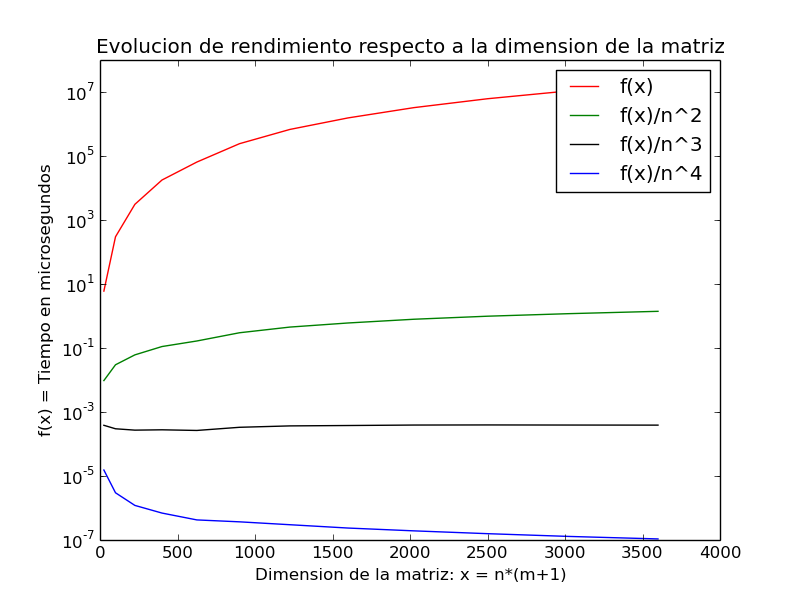
\includegraphics[scale=0.35]{experimentos2a_2b/tiempos_nm_fitteo_1_inst/eliminacion_gaussiana_time_consumed.png}
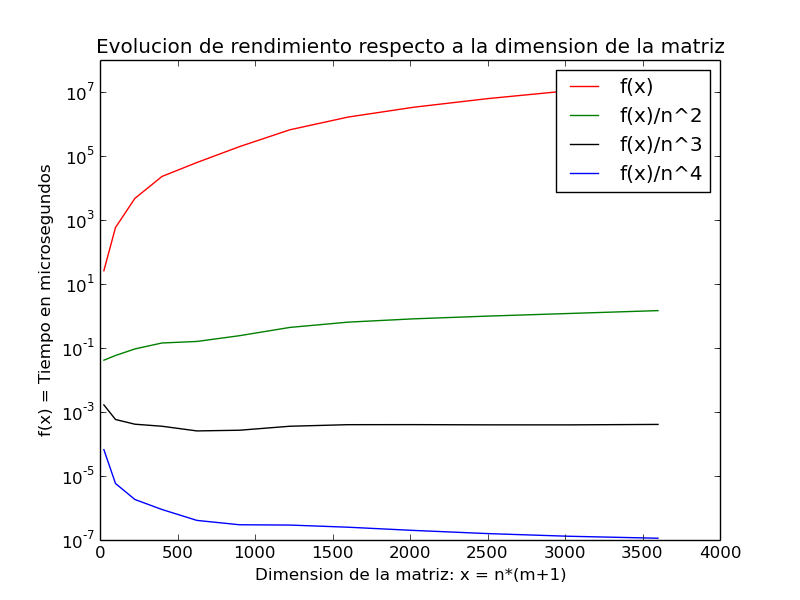
\includegraphics[scale=0.35]{experimentos2a_2b/tiempos_nm_fitteo_1_inst/factorizacion_lu_time_consumed.png}
\end{center}

A pesar de ser una heur\'istica, podemos corroborar que la curva sobre cubo se asemeja mucho a una constante, mientras que al cuadrado y a la cuarta funciones crecientes y decrecientes, respectivamente. Por lo que podemos decir que probamos emp\'iricamente que los algoritmos son del orden c\'ubico.

\subsubsection{Performance de EG vs LU variando la cantidad de instancias y la granularidad de la discretizacion}

Para comenzar esta seccion, compararemos la performance de EG vs LU variando las discretizaciones, con archivos de entrada de una sola instancia. A continuacion se presentan los graficos de comparación entre EG y LU, en diferentes escalas.

\begin{center}
\textbf{1 instancia por archivo de test}\\
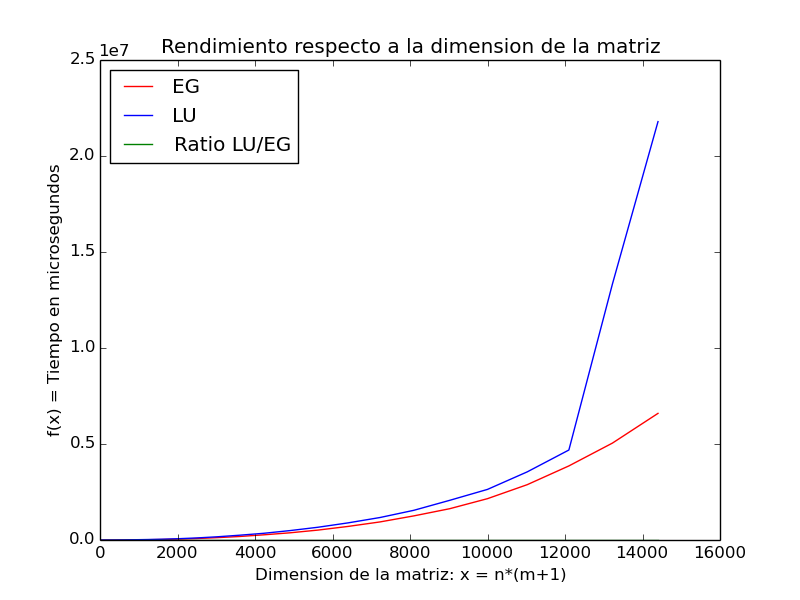
\includegraphics[scale=0.35]{experimentos2a_2b/tiempos_nm_fitteo_1_inst/gauss_vs_lu_time_consumed_abs.png}
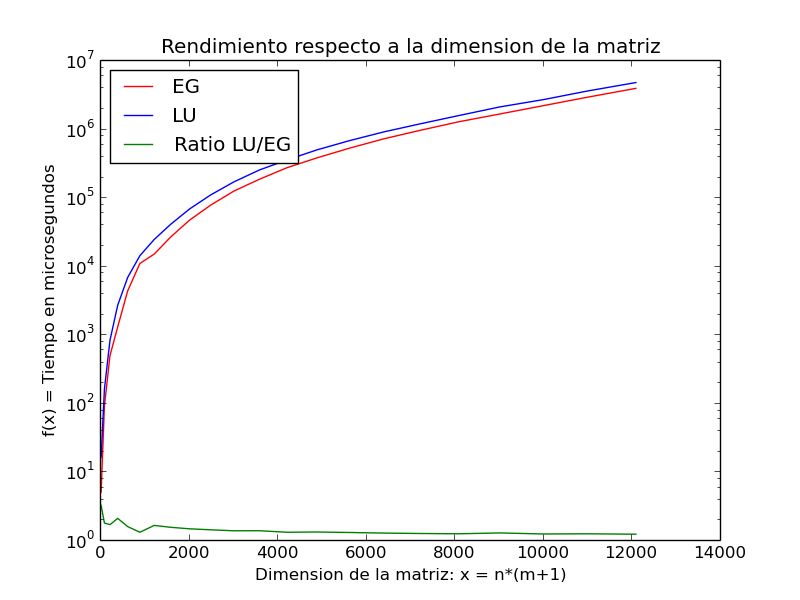
\includegraphics[scale=0.35]{experimentos2a_2b/tiempos_nm_fitteo_1_inst/gauss_vs_lu_time_consumed_log.png}
\end{center}

Dado que factorizacion LU, es identico a EG, pero guardando los coeficientes en la matriz L, tiene sentido que para una sola instancia sea mas costoso realizar la factorizacion lu y resolver el sistema que simplemente resolver usando EG.

\vspace{0.5cm}

A continuacion, se presentan graficos comparativos entre LU y EG para distintas cantidades de instancias. Lo que se observa es que, la brecha entre EG y LU se acentúa cada vez más a medida que aumenta la cantidad de instancias(ver gráficos con escala lineal). Esto se debe a que la complejidad teorica de resolver k instancias (misma matriz A, distinto vector b, en un sistema Ax=b) usando EG es $\mathcal{O}( k * (n + m)^3 )$. Por otro lado, la complejidad de resolver k instancias usando LU es $\mathcal{O}((n + m)^3 + k*(n + m)^2)$, es decir: Complejidad cúbica para hallar la descomposicion LU, y luego $k$ resoluciones de los sistemas triangulares $Ly=b$ y $Ux=y$ que cuestan orden cuadrático cada uno. 

\begin{center}
\textbf{10 instancias por archivo de test}\\
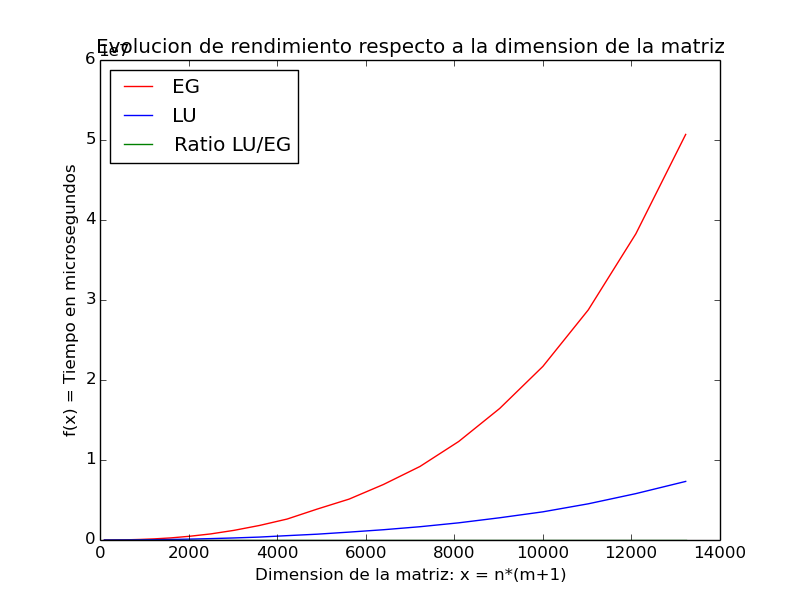
\includegraphics[scale=0.35]{experimentos2a_2b/gauss_vs_lu_10_inst/gauss_vs_lu_time_consumed_abs.png}
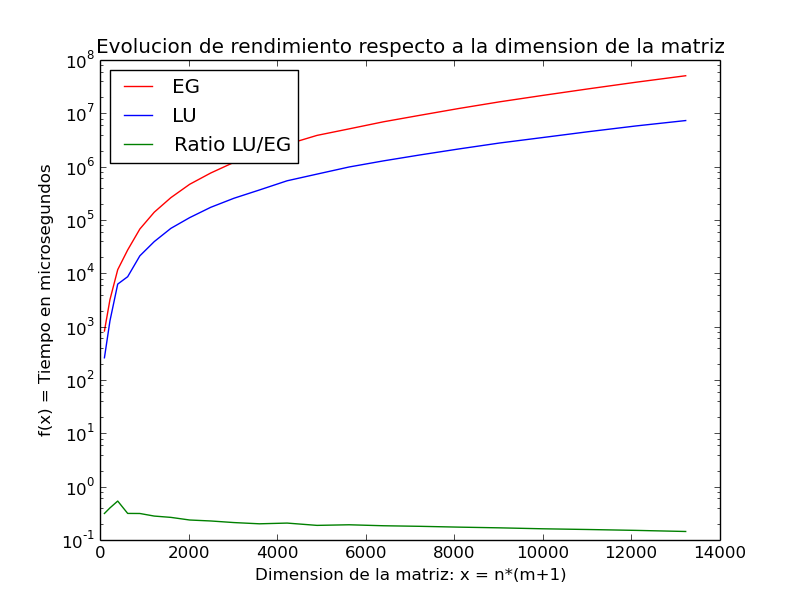
\includegraphics[scale=0.35]{experimentos2a_2b/gauss_vs_lu_10_inst/gauss_vs_lu_time_consumed_log.png}
\end{center}

\begin{center}
\textbf{50 instancias por archivo de test}\\
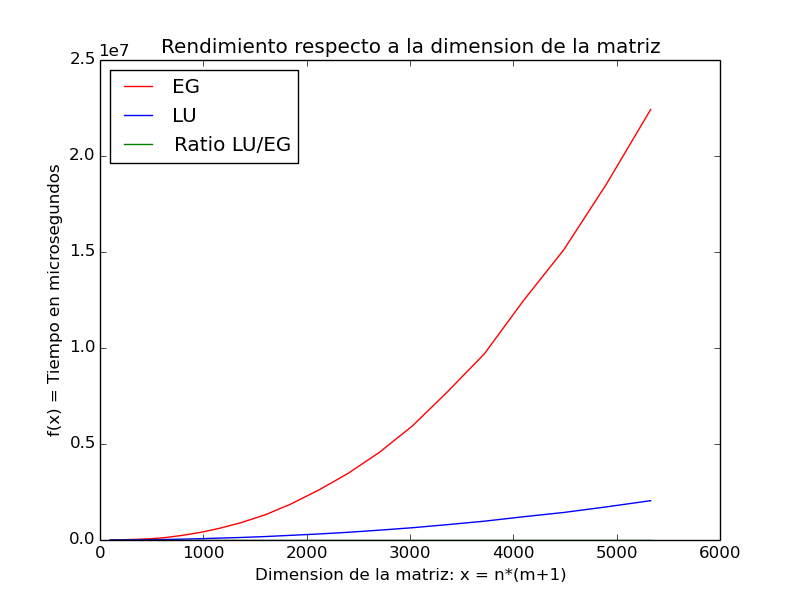
\includegraphics[scale=0.35]{experimentos2a_2b/gauss_vs_lu_50_inst/gauss_vs_lu_time_consumed_abs.png}
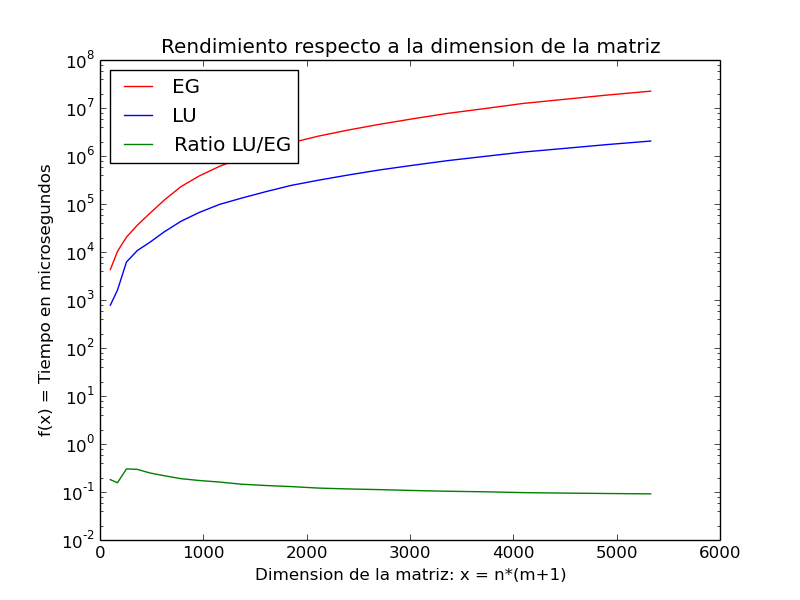
\includegraphics[scale=0.35]{experimentos2a_2b/gauss_vs_lu_50_inst/gauss_vs_lu_time_consumed_log.png}
\end{center}

\begin{center}
\textbf{150 instancias por archivo de test}\\
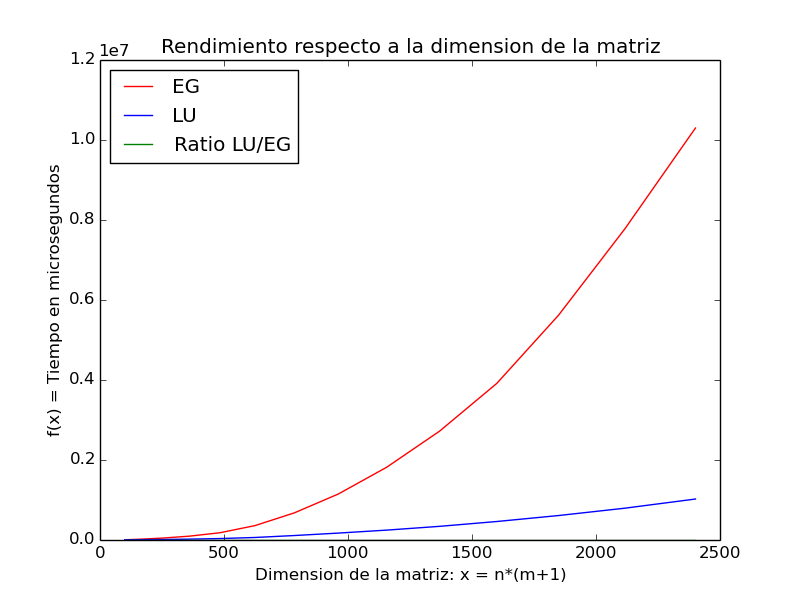
\includegraphics[scale=0.35]{experimentos2a_2b/gauss_vs_lu_150_inst/gauss_vs_lu_time_consumed_abs.png}
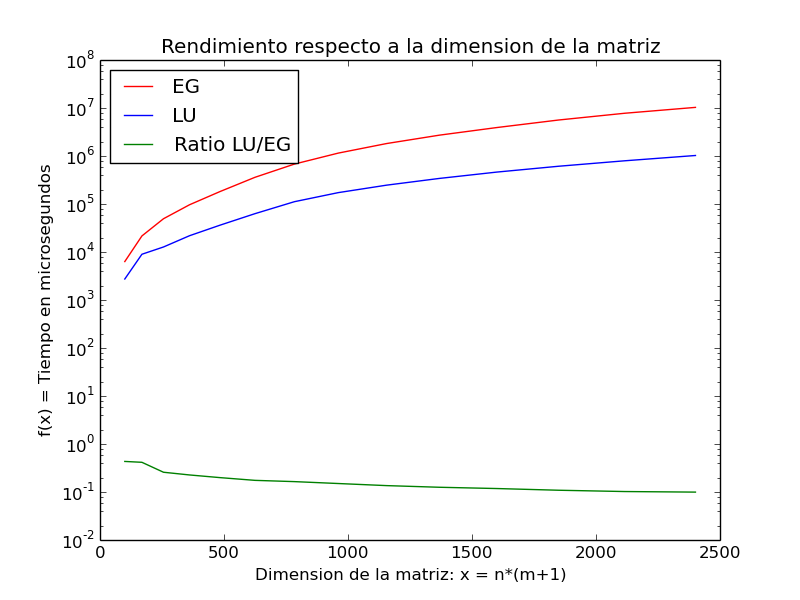
\includegraphics[scale=0.35]{experimentos2a_2b/gauss_vs_lu_150_inst/gauss_vs_lu_time_consumed_log.png}
\end{center}

\begin{center}
\textbf{500 instancias por archivo de test}\\
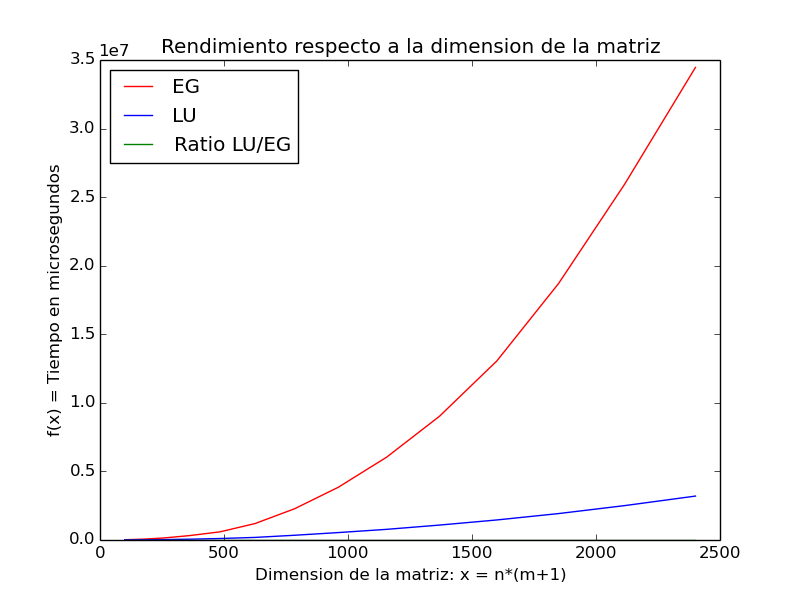
\includegraphics[scale=0.35]{experimentos2a_2b/gauss_vs_lu_500_inst/gauss_vs_lu_time_consumed_abs.png}
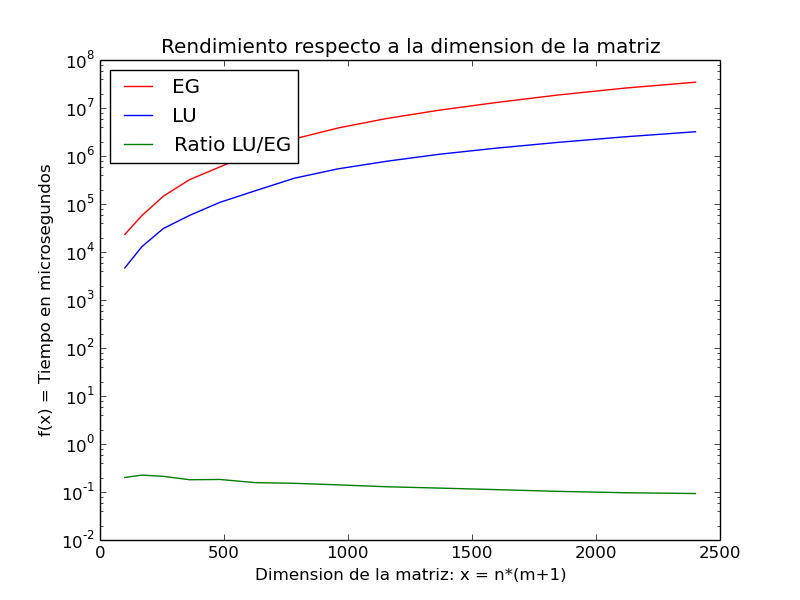
\includegraphics[scale=0.35]{experimentos2a_2b/gauss_vs_lu_500_inst/gauss_vs_lu_time_consumed_log.png}
\end{center}

Tambien se observa en los graficos con escala logaritmica que la brecha entre EG y LU para una cantidad de instancias fija se acentua a medida que se aumenta el tamaño de la matriz del sistema, pues el ratio LU/EG decrece. Creemos que esto se debe a que al dejar k fijo y aumentar $n+m$, tenemos que $\mathcal{O}((n + m)^3 + k*(n + m)^2)$ es mas pequeño que $\mathcal{O}(k*(n + m)^3)$ en terminos empíricos. 

\textbf{Consideraci\'on Adicional:} 

Luego de la experimentacion, se nos ocurrio una optimizacion de la implementaci\'on de los algoritmos, se agreg\'o la siguiente sentencia condicional al código de EG y la parte de triangulacion de LU:

\begin{lstlisting}
			.
			.
			.
for (int j = i+1; j < numfilas; j++) {

            if (abs(_A[j][i]) < EPSILON) {
                continue;
            }
			.
			.
			.
\end{lstlisting}

Es decir, si el elemento a analizar de la matriz es un cero(con tolerancia epsilon, en nuestro caso $exp(10, -9)$), el algoritmo no realiza el c\'alculo del coeficiente multiplicador ni tampoco opera sobre la fila multiplicando cada elemento por \'este. Al agregar esta sentencia y realizar los experimentos de fitteo de orden de complejidad, obtuvimos como resultado que la complejidad emp\'irica de ambos algoritmos era de orden cuadr\'atico. Creemos que esto se debe a la condición banda de la matriz, y que en muchos casos esta condición de corte evita que el algoritmo ingrese en la tercera iteracion anidada.

\subsection{Diferencia numérica de soluciones entre EG y LU}
En esta sección se mostraran los resultados de comparar las soluciones a un mismo sistema de ecuaciones $Ax=b$ usando LU y EG. Se realizo una variación en el tamaño de la matriz del sistema para ver la evolucion de las mediciones.\\

\vspace{0.3cm}

Los parámetros utilizados para el experimento fueron:
\begin{itemize}
	\item \textbf{Temperaturas internas y externas:}  externas(1500) e internas(100) \textbf{constantes} en todos los tests. 
	\item \textbf{Radio interno:} 200
	\item \textbf{Radio externo:} 400
	\item \textbf{Tamaño n de la matriz $A \in \mathbb{R}^{n \times n}$:} $[10^2\dots130^2]$
	\item \textbf{Isoterma buscada:} 500
\end{itemize}

No se mostrará ningun gráfico porque todas las mediciones de diferencia dieron cero, es decir:

\begin{itemize}
    \item $\norm{ x - \hat{x} }_\infty = 0.0 $
    \item $\norm{ x - \hat{x} }_2 = 0.0 $ 
\end{itemize}

Dado este sorprendente resultado a primera vista, hicimos un análisis mas fino del codigo y llegamos a algunas conclusiones:
\begin{itemize}
	\item El código de la resolución del problema es identico en ambos métodos desde la lectura de la entrada hasta el armado del sistema $Ax=b$, con lo cual no puede haber diferencia numérica en este tramo.
	\item El código de factorizacion lu y eliminacion gaussiana es \texttt{idéntico} salvo que LU guarda los multiplicadores en otra matriz L, tambien de precision doble, con lo cual lo único que podria acarrear LU contra EG en este tramo es el almacenamiento con error de los coeficientes.
	\item LU tambien podría acarrear error al realizar las 2 resoluciones de sistemas triangulares(contra una sola de EG)
\end{itemize}

Sin embargo, en los casos planteados esto no ocurre. Como futuro trabajo, se podrian fabricar casos de test muy especificos donde se fuercen errores numericos clásicos. (ie. sumas con números de distinto orden, restas con numeros muy cercanos, etc.) en las operaciones de resolucion de los sistemas triangulares, se esperaría que LU acarree mas error ya que realiza mas operaciones para resolver el sistema original $Ax=b$.

\subsection{Evolución estimación de la isoterma y temperatura}
Se presentarán los resultados de los experimentos en el mismo orden en que fueron planteados en la sección de desarrollo. Se realizará el análisis de los mismos en este mismo apartado.
\begin{enumerate}
	\item \begin{itemize}
				\item \textbf{Temperaturas internas y externas:} aleatorias uniformes entre $[50\dots200]$ y $[1450\dots1550]$, pero fijas entre tests.
				\item \textbf{Radio interno:} 200
				\item \textbf{Radio externo:} 400
				\item \textbf{Cantidad radios:} $[5\dots100]$
				\item \textbf{Cantidad ángulos:} 100
				\item \textbf{Isoterma buscada:} 500
			\end{itemize}
Se adjunta con el trabajo práctico un video que expone la evolución del sistema mientras se incrementa la cantidad de radios. Expondremos estáticamente algunos frames, pero es conveniente ver el video primero. Se encuentra en la misma carpeta que el pdf. (variación\_radial\_isomap.mp4, variación\_radial\_heatmap.mp4).

\vspace{0.5cm}

  	\textbf{Variación de la estimación de la isoterma entre 5 y 6 radios de discretización}\\
	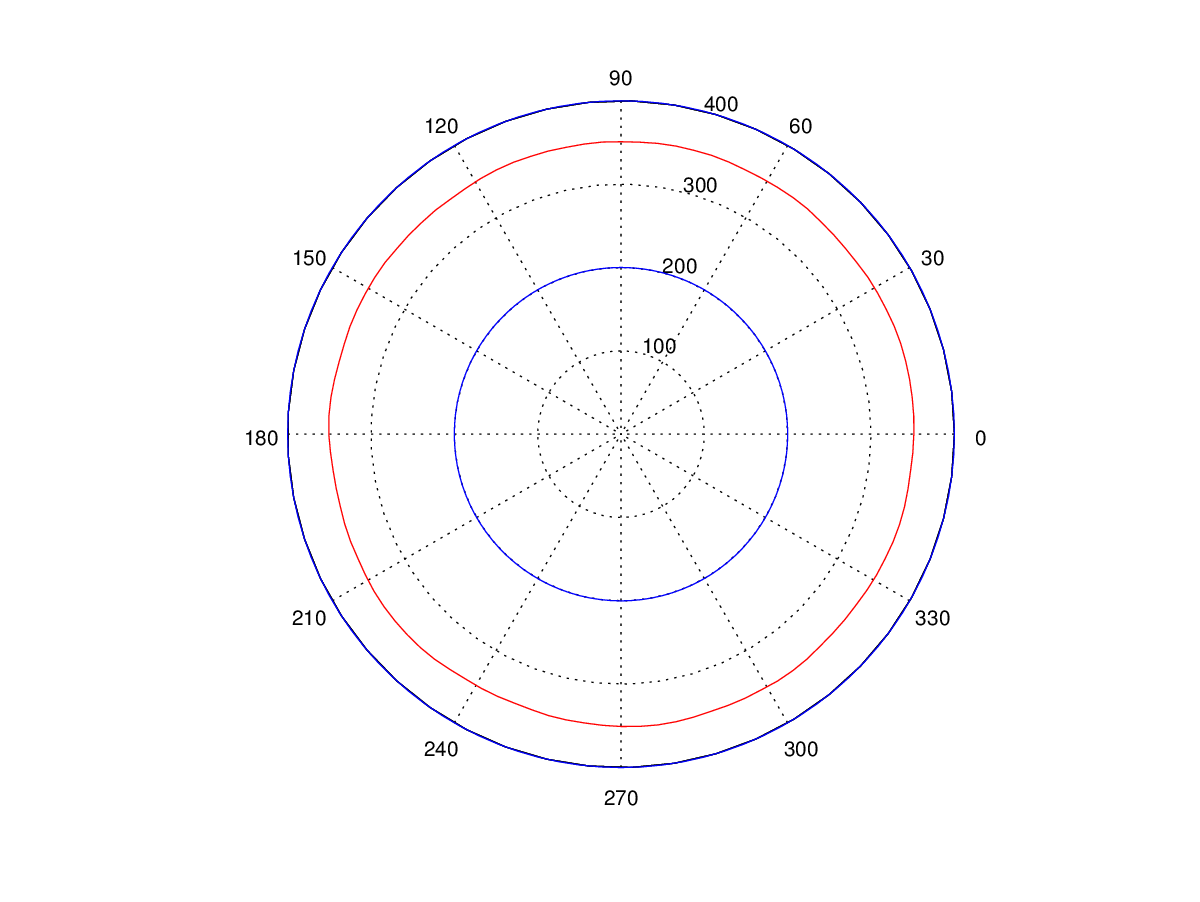
\includegraphics[scale=0.35]{experimentos1a_1b/evolucion_posicion_isoterma_temperatura/test2/test6_006_radios_inst_001_isomap.png}
	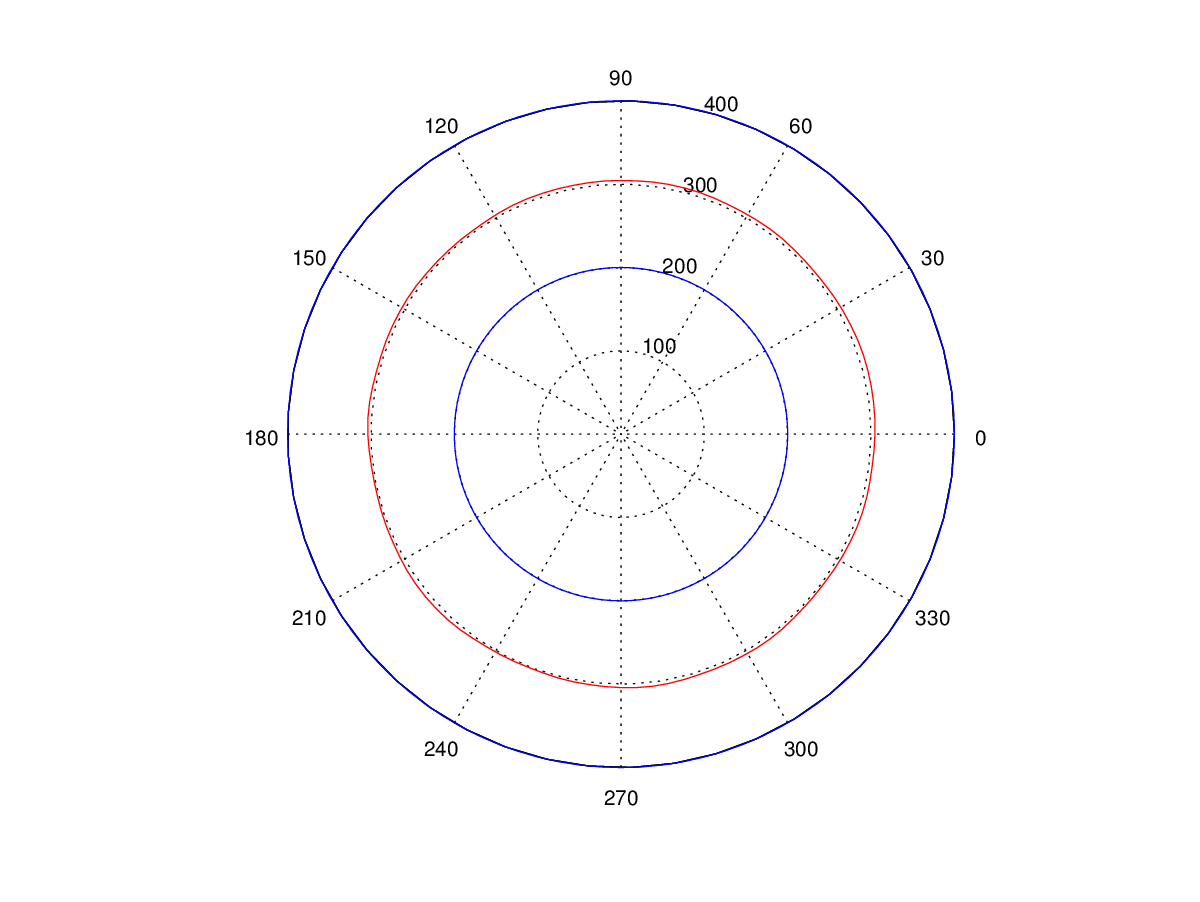
\includegraphics[scale=0.35]{experimentos1a_1b/evolucion_posicion_isoterma_temperatura/test2/test6_007_radios_inst_001_isomap.png}
	
  	\textbf{Variación de la temperatura entre 6 y 7 radios de discretización}\\
	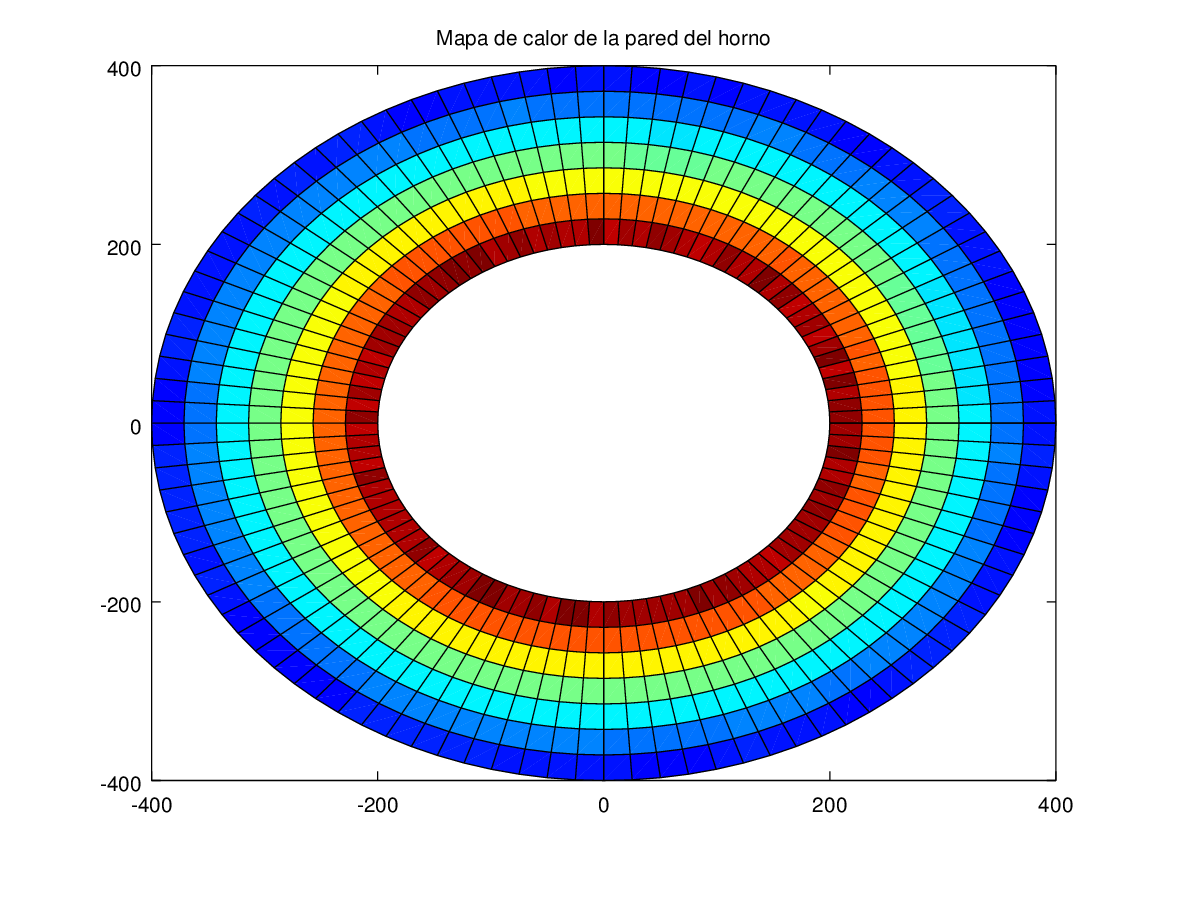
\includegraphics[scale=0.35]{experimentos1a_1b/evolucion_posicion_isoterma_temperatura/test2/test6_006_radios_inst_001_heatmap.png}
	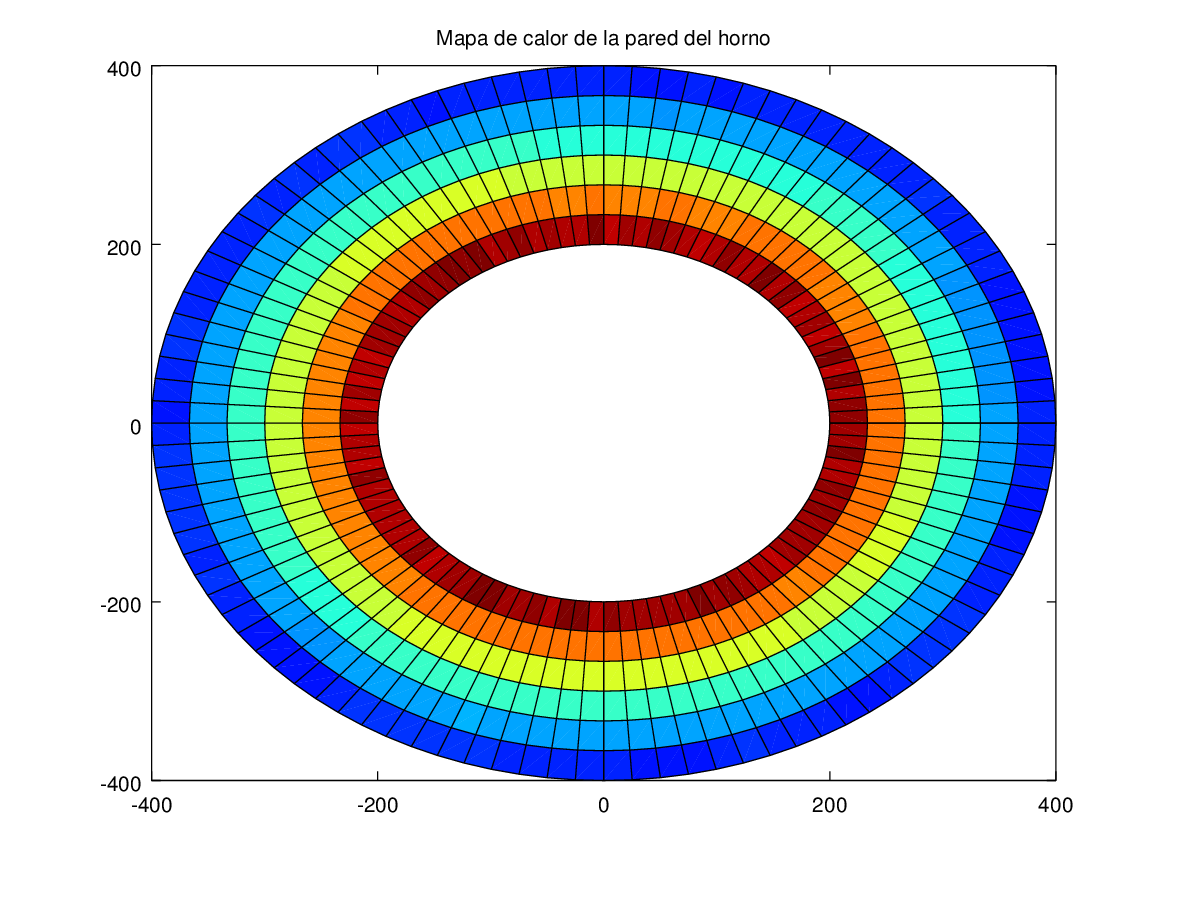
\includegraphics[scale=0.35]{experimentos1a_1b/evolucion_posicion_isoterma_temperatura/test2/test6_007_radios_inst_001_heatmap.png}

 	\textbf{Variación de la estimación de la isoterma entre 99 y 100 radios de discretización}\\
	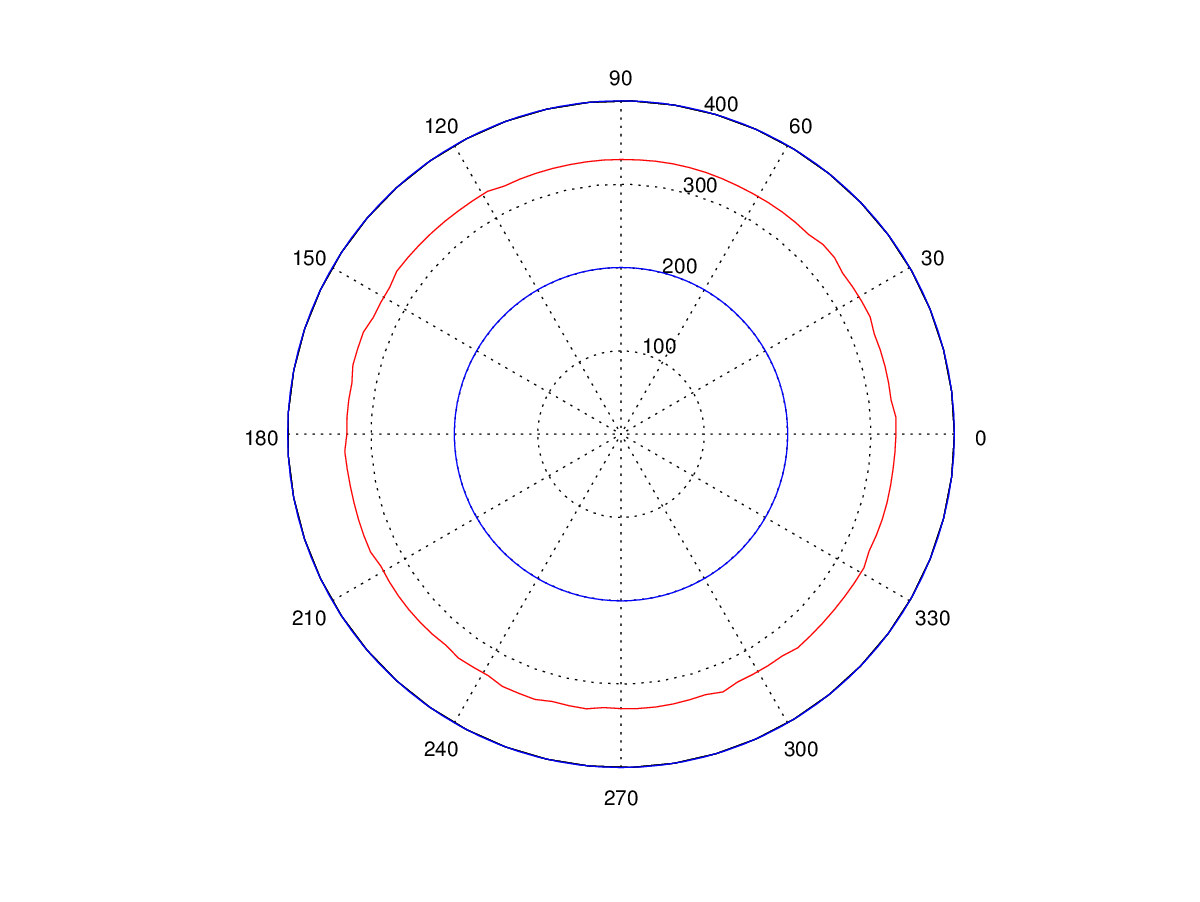
\includegraphics[scale=0.35]{experimentos1a_1b/evolucion_posicion_isoterma_temperatura/test2/test6_099_radios_inst_001_isomap.png}
	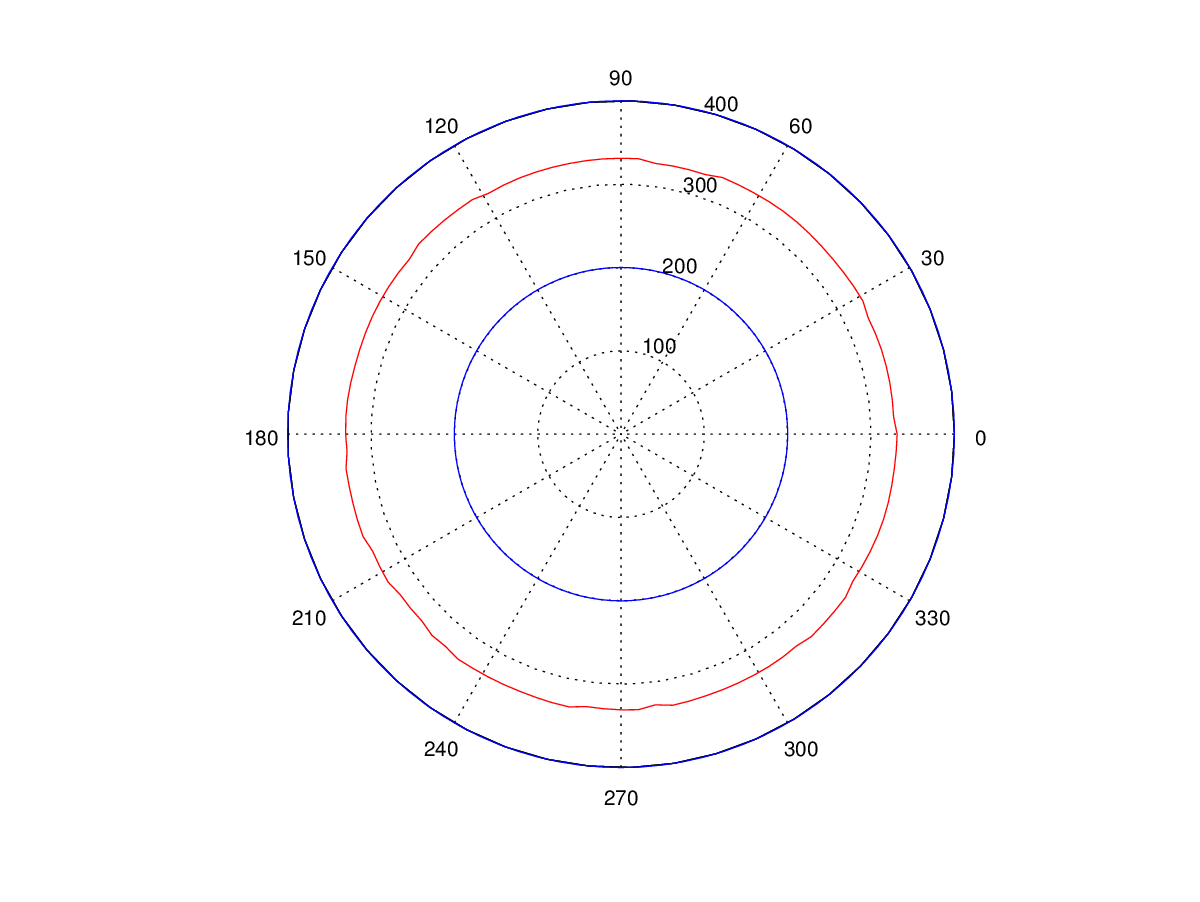
\includegraphics[scale=0.35]{experimentos1a_1b/evolucion_posicion_isoterma_temperatura/test2/test6_100_radios_inst_001_isomap.png}
	
	\textbf{Variación de la temperatura entre 99 y 100 radios de discretización}\\
	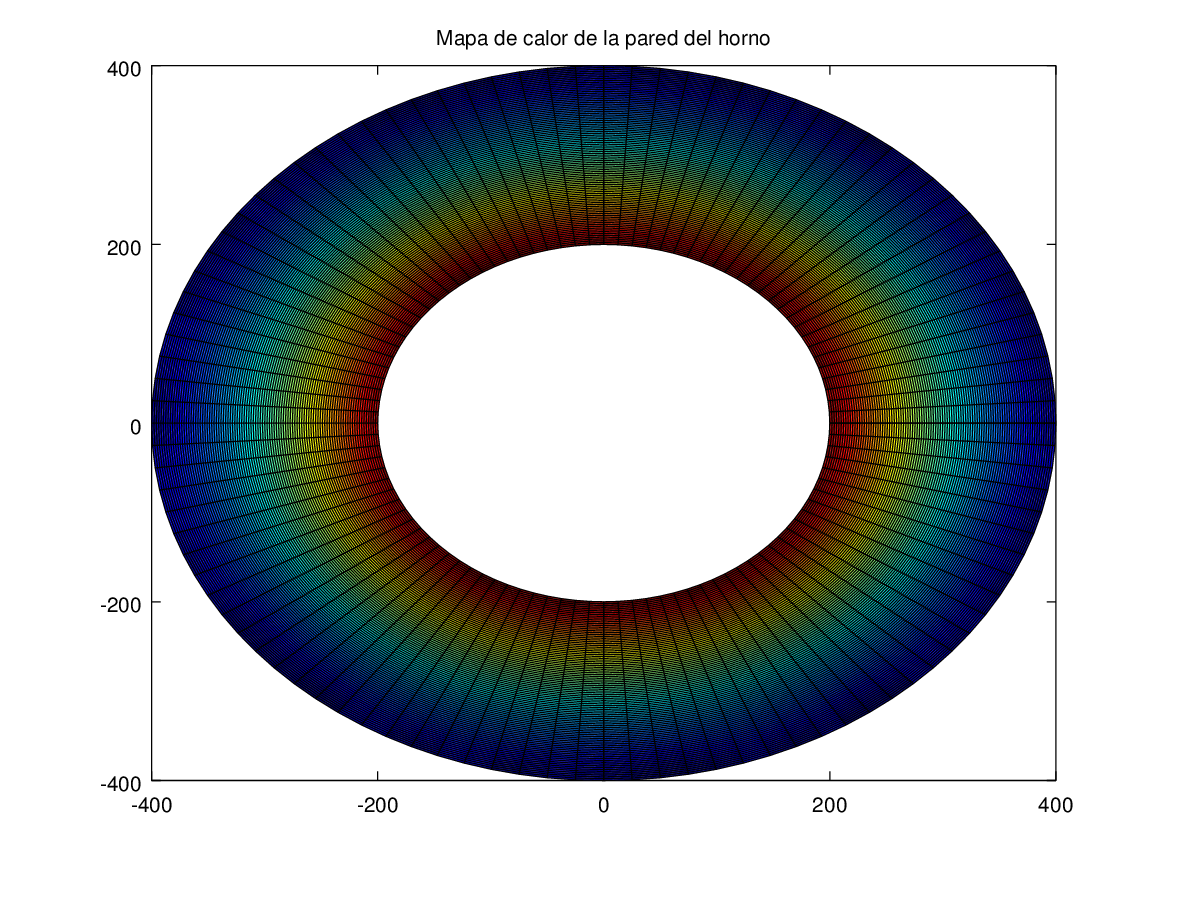
\includegraphics[scale=0.35]{experimentos1a_1b/evolucion_posicion_isoterma_temperatura/test2/test6_099_radios_inst_001_heatmap.png}
	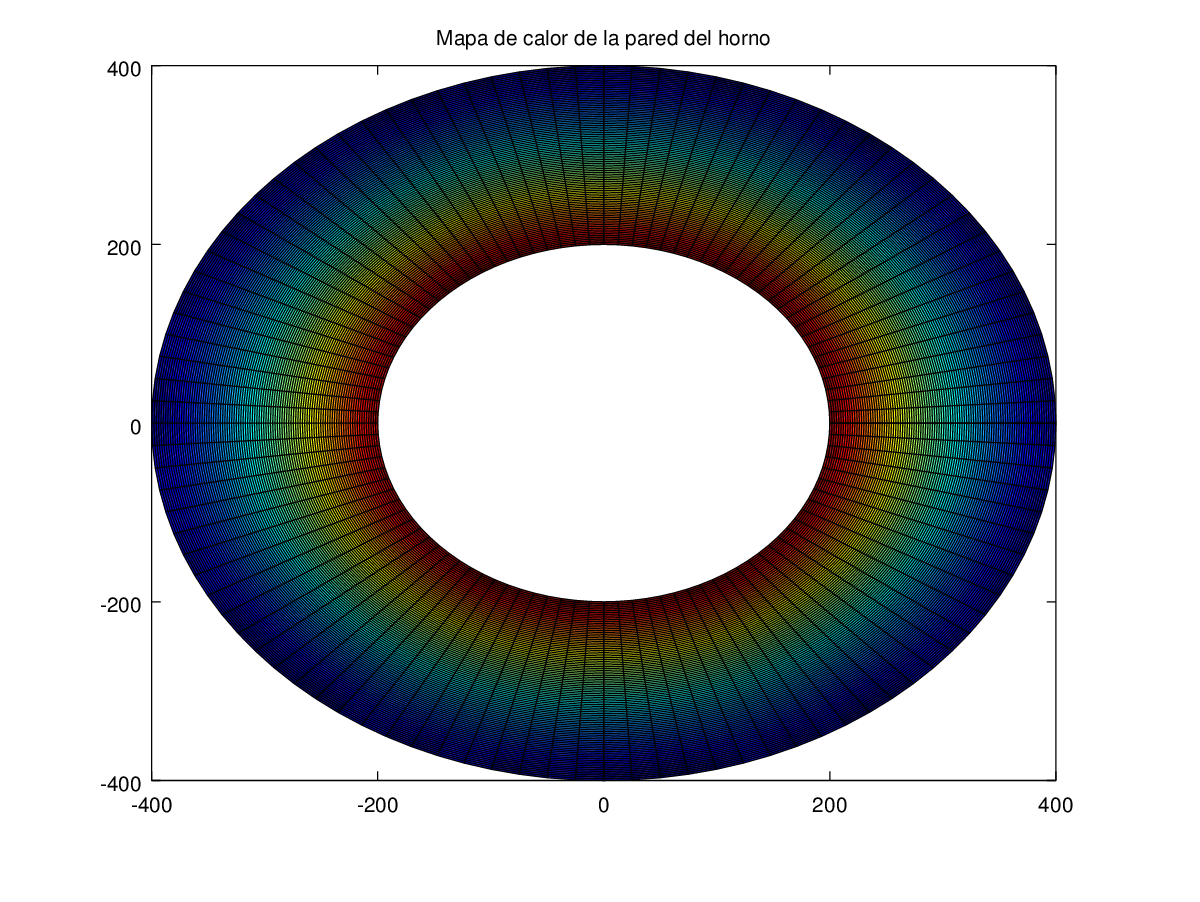
\includegraphics[scale=0.35]{experimentos1a_1b/evolucion_posicion_isoterma_temperatura/test2/test6_100_radios_inst_001_heatmap.png}

\vspace{0.5cm}

Se observa es que a medida que se aumenta la cantidad de radios de la discretización, la variación radial de la curva de la isoterma disminuye entre tests, es decir, se hace más fina la estimación, de forma tal que entre $i$ e $i+1$ radios la diferencia de la posición de la isoterma es menor a medida que $i$ crece. Para ver mejor esto se graficaron, para cada test de $i$ cantidad de radios de la discretización, el máximo y el promedio radial de la isoterma.

	\textbf{Evolución de la variación radial de la isoterma con cantidad creciente de radios}\\
	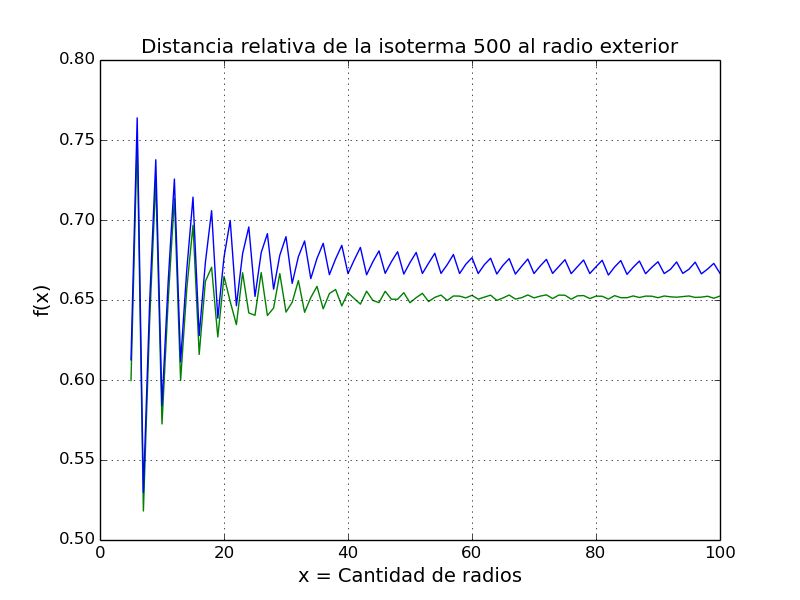
\includegraphics[scale=0.5]{experimentos1a_1b/evolucion_estimacion_seguridad_isoterma/100ang_5to100radios.png}\\


Para evitar distorsiones en el experimento anterior, se realizo otro muy similar al anterior pero con condiciones de borde \textbf{constantes e iguales}.
\begin{itemize}
	\item \textbf{Temperaturas internas y externas:} constantes, 100 y 1500. Esto es para que tenga la misma solución cada test del experimento.
	\item \textbf{Radio interno:} 200
	\item \textbf{Radio externo:} 400
	\item \textbf{Cantidad radios:} $[10\dots200]$
	\item \textbf{Cantidad ángulos:} 75
	\item \textbf{Isoterma buscada:} 500
\end{itemize}

No expondremos los resultados acerca de la evolucion de la temperatura y posicion de la isoterma, pues son similares al experimento anterior, la isoterma converge a medida que aumenta la cantidad de radios utilizada en la discretización. Al ser temperaturas constantes en este caso, la isoterma es un círculo perfecto. En el experimento anterior, la isoterma tenia pequeñas(casi imperceptibles) irregularidades dadas las condiciones aleatorias(con baja varianza) de borde.

\vspace{0.3cm}

Respecto al gráfico del promedio/maximo de la isoterma a medida que aumentan los radios, se tiene lo siguiente.

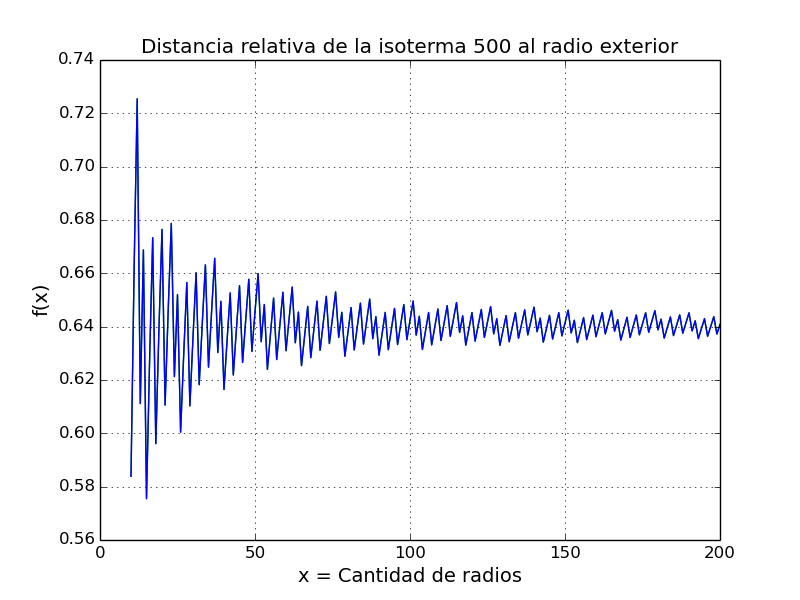
\includegraphics[scale=0.5]{experimentos1a_1b/evolucion_estimacion_seguridad_isoterma/75ang_10to200rad_evol_maxpromradio.png}\\
\textbf{Nota:} Al ser las condiciones de borde iguales, la isoterma tiene radio constante para cada experimento, con lo cual maximo y promedio coinciden, con lo cual se ve una sola curva.

\vspace{0.2cm}

Se puede ver que, al igual que en el experimento anterior, al aumentar la cantidad de radios, la posicion de la isoterma converge. Tambien se observa que en ambos experimentos, la posicion relativa de la isoterma converge aproximadamente a 0.64/0.66, lo cual tiene sentido ya que el experimento anterior tenia temperaturas aleatorias uniformes, pero \texttt{casi} alrededor de las temperaturas fijadas en el segundo experimento.\\

	\item \begin{itemize}
					\item \textbf{Temperaturas internas y externas:} constantes, 100 y 1500. Esto es para que tenga la misma solución cada test del experimento.
					\item \textbf{Radio interno:} 200
					\item \textbf{Radio externo:} 400
					\item \textbf{Cantidad radios:} 50
					\item \textbf{Cantidad ángulos:} $[5\dots50]$
					\item \textbf{Isoterma buscada:} 500
				\end{itemize}
	Se adjunta con el trabajo práctico un video que expone la evolución del sistema mientras se incrementa la cantidad de radios. Expondremos estáticamente algunos frames, pero es conveniente ver el video primero. Se encuentra en la misma carpeta que el pdf. (variación\_angular\_isomap.mp4, variación\_angular\_heatmap.mp4).

	\vspace{0.5cm}
	  	\textbf{Variación de la estimación de la isoterma entre 5 y 6 ángulos de discretización}\\
		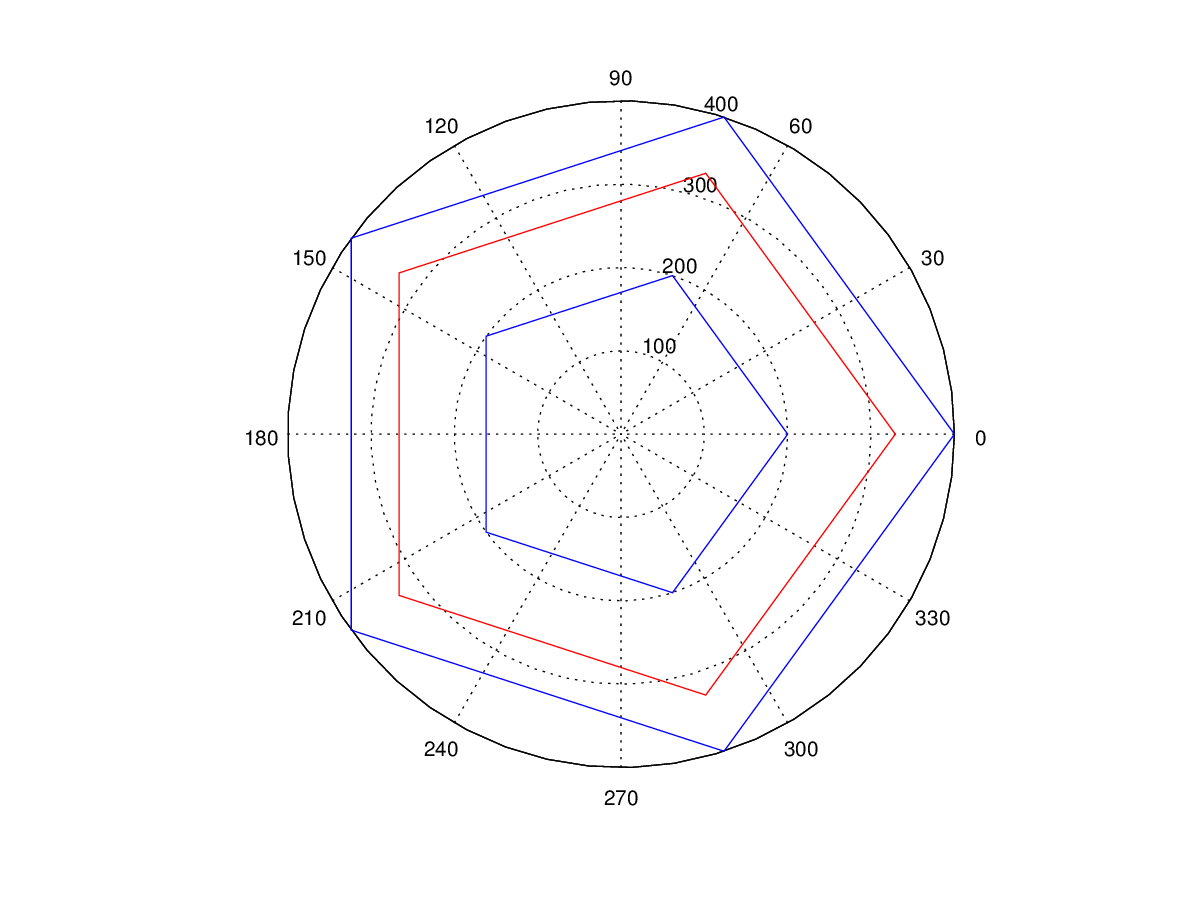
\includegraphics[scale=0.35]{experimentos1a_1b/evolucion_posicion_isoterma_temperatura/variacion_angulos_radio_fijo_se_suaviza_isoterma/test10_050_radios_005_angulos_inst_001_isomap.png}
		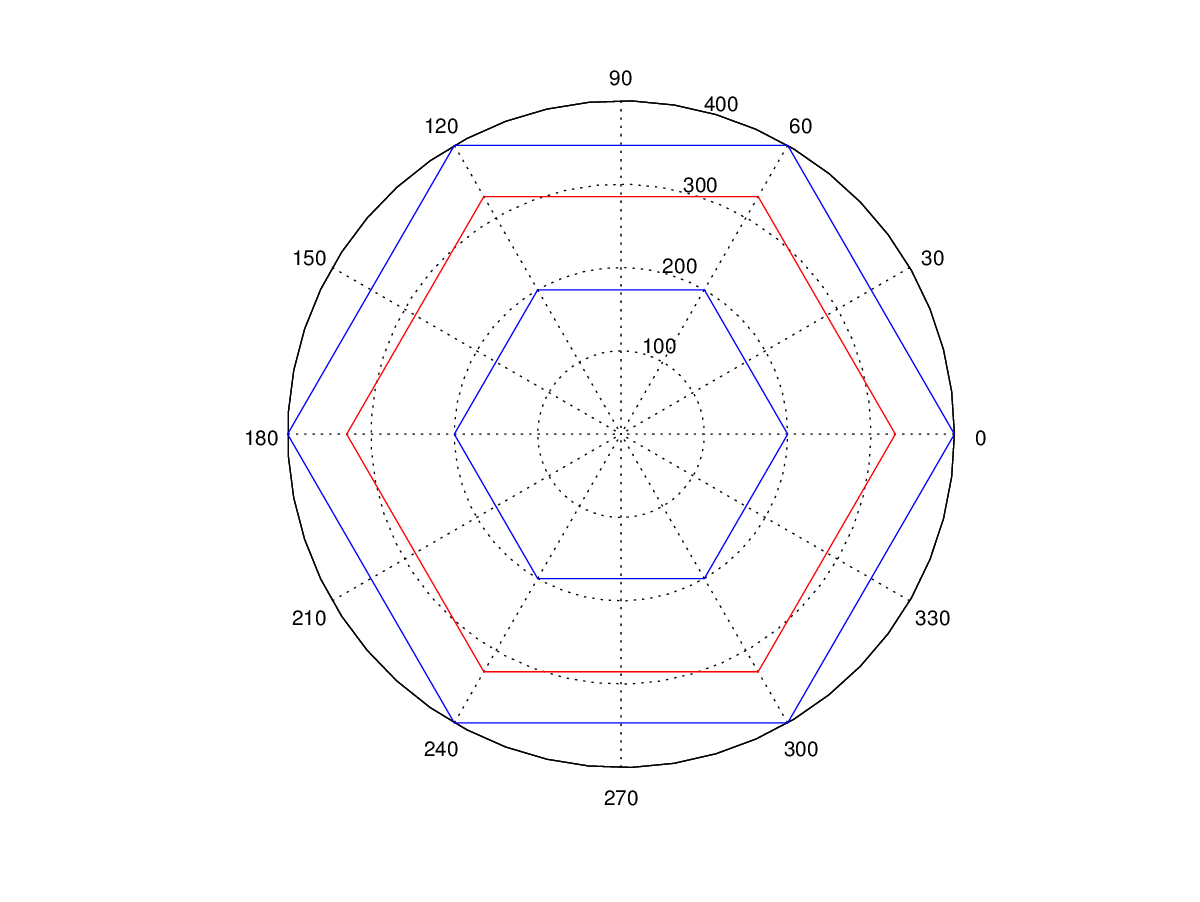
\includegraphics[scale=0.35]{experimentos1a_1b/evolucion_posicion_isoterma_temperatura/variacion_angulos_radio_fijo_se_suaviza_isoterma/test10_050_radios_006_angulos_inst_001_isomap.png}

	  	\textbf{Variación de la temperatura entre 5 y 6 ángulos de discretización}\\
	  	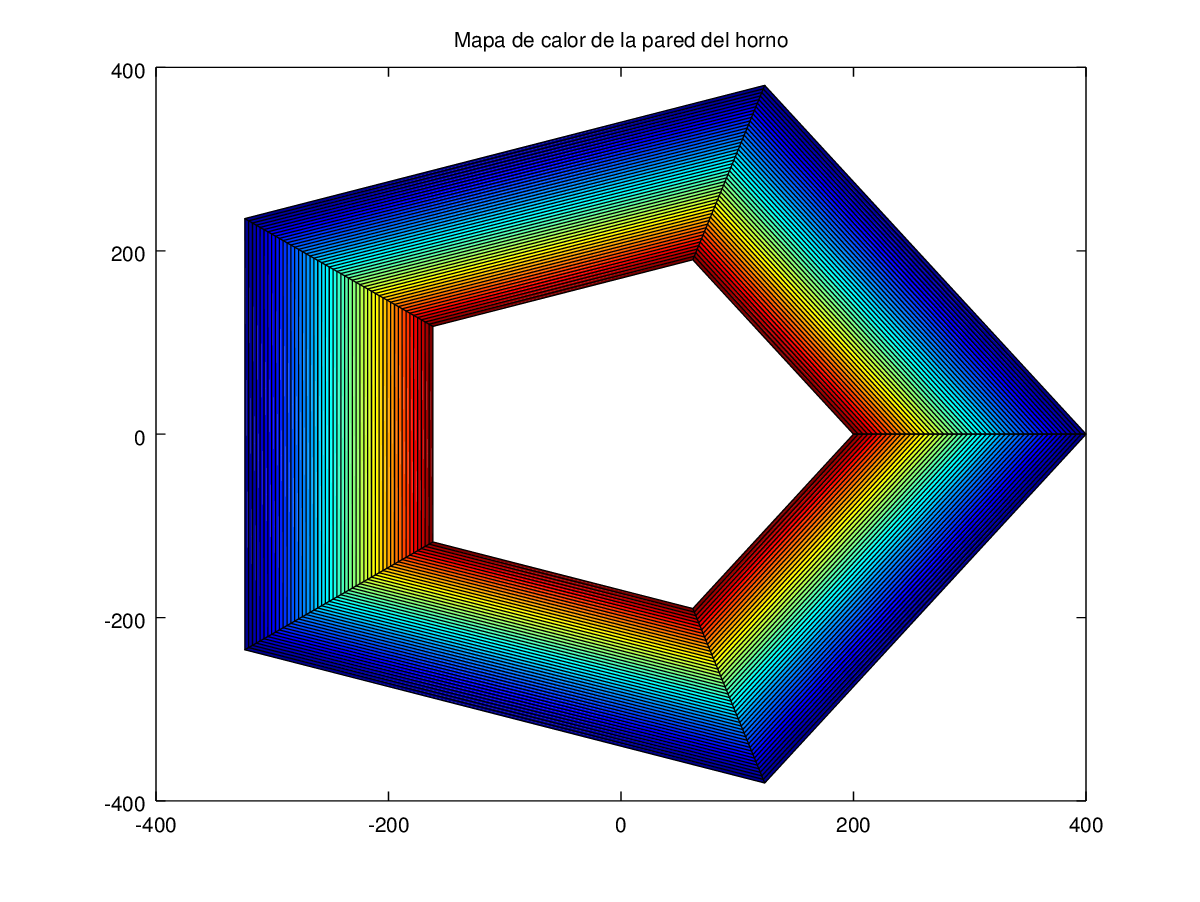
\includegraphics[scale=0.35]{experimentos1a_1b/evolucion_posicion_isoterma_temperatura/variacion_angulos_radio_fijo_se_suaviza_isoterma/test10_050_radios_005_angulos_inst_001_heatmap.png}
		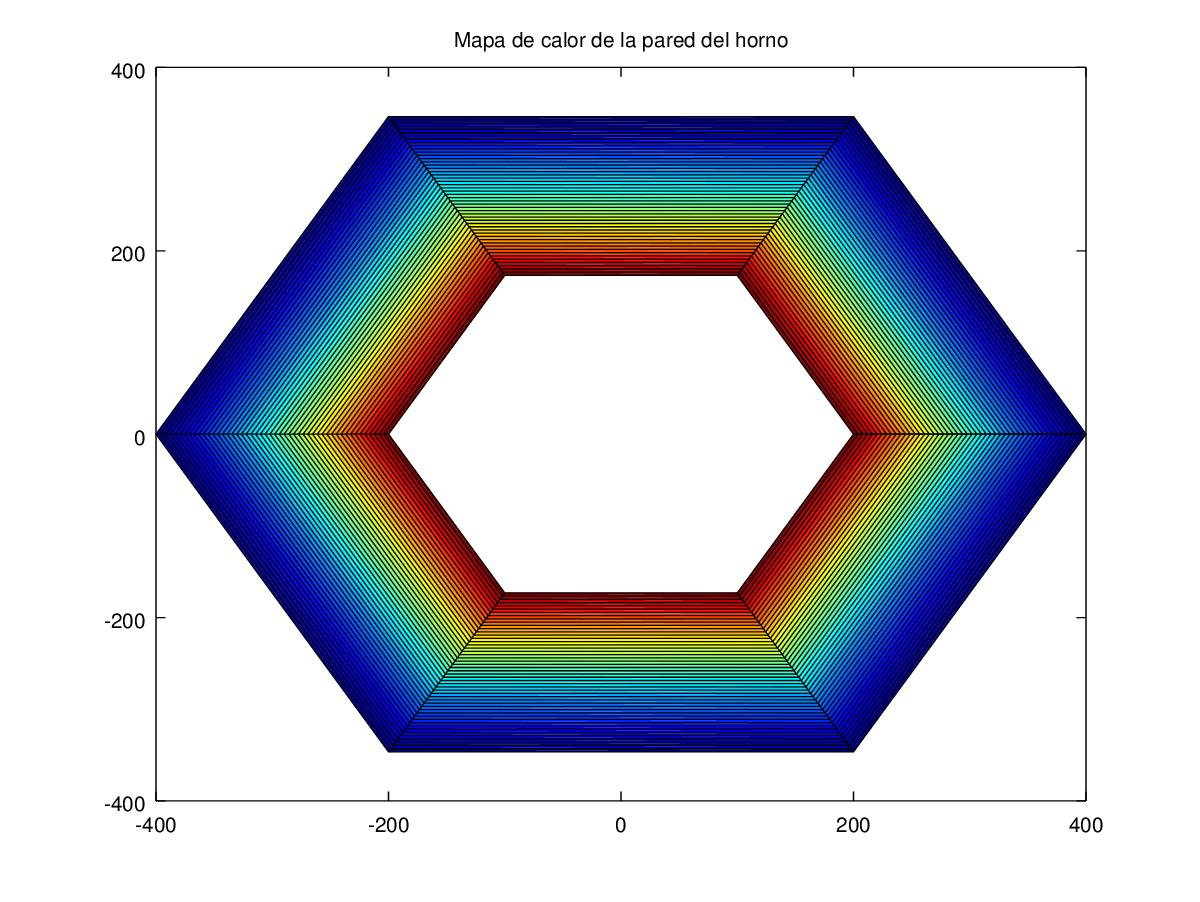
\includegraphics[scale=0.35]{experimentos1a_1b/evolucion_posicion_isoterma_temperatura/variacion_angulos_radio_fijo_se_suaviza_isoterma/test10_050_radios_006_angulos_inst_001_heatmap.png}	  	

	  	\textbf{Variación de la estimación de la isoterma entre 49 y 50 ángulos de discretización}\\
		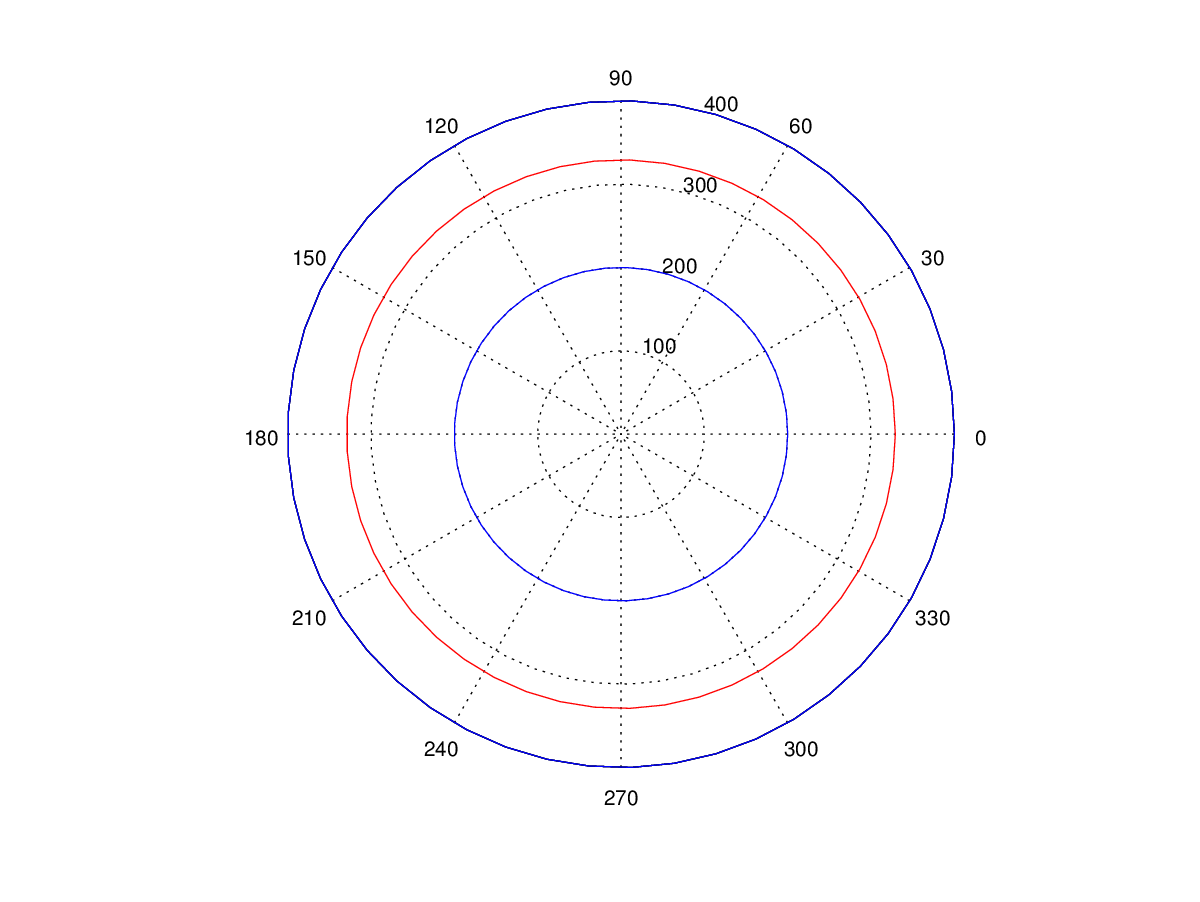
\includegraphics[scale=0.35]{experimentos1a_1b/evolucion_posicion_isoterma_temperatura/variacion_angulos_radio_fijo_se_suaviza_isoterma/test10_050_radios_049_angulos_inst_001_isomap.png}
		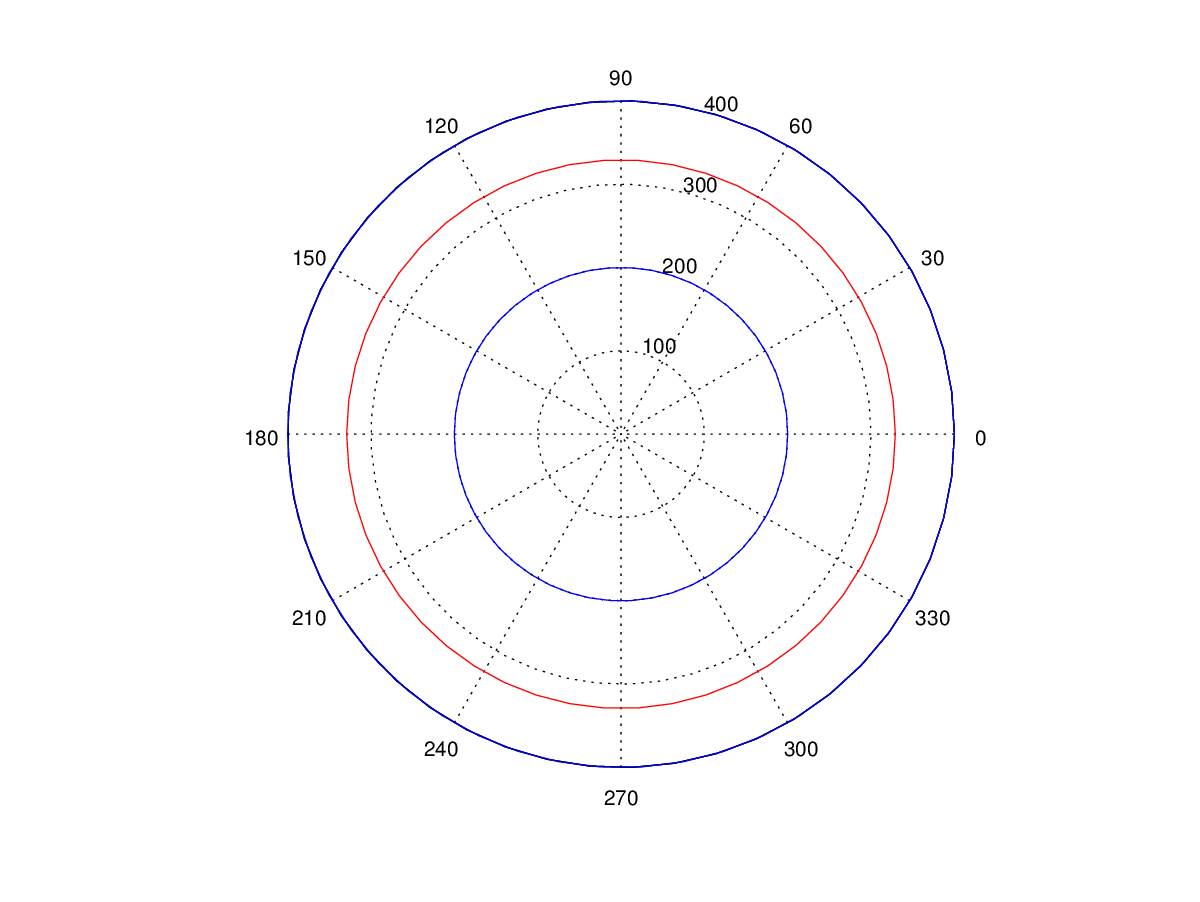
\includegraphics[scale=0.35]{experimentos1a_1b/evolucion_posicion_isoterma_temperatura/variacion_angulos_radio_fijo_se_suaviza_isoterma/test10_050_radios_050_angulos_inst_001_isomap.png}

		\textbf{Variación de la temperatura entre 49 y 50 ángulos de discretización}\\
	  	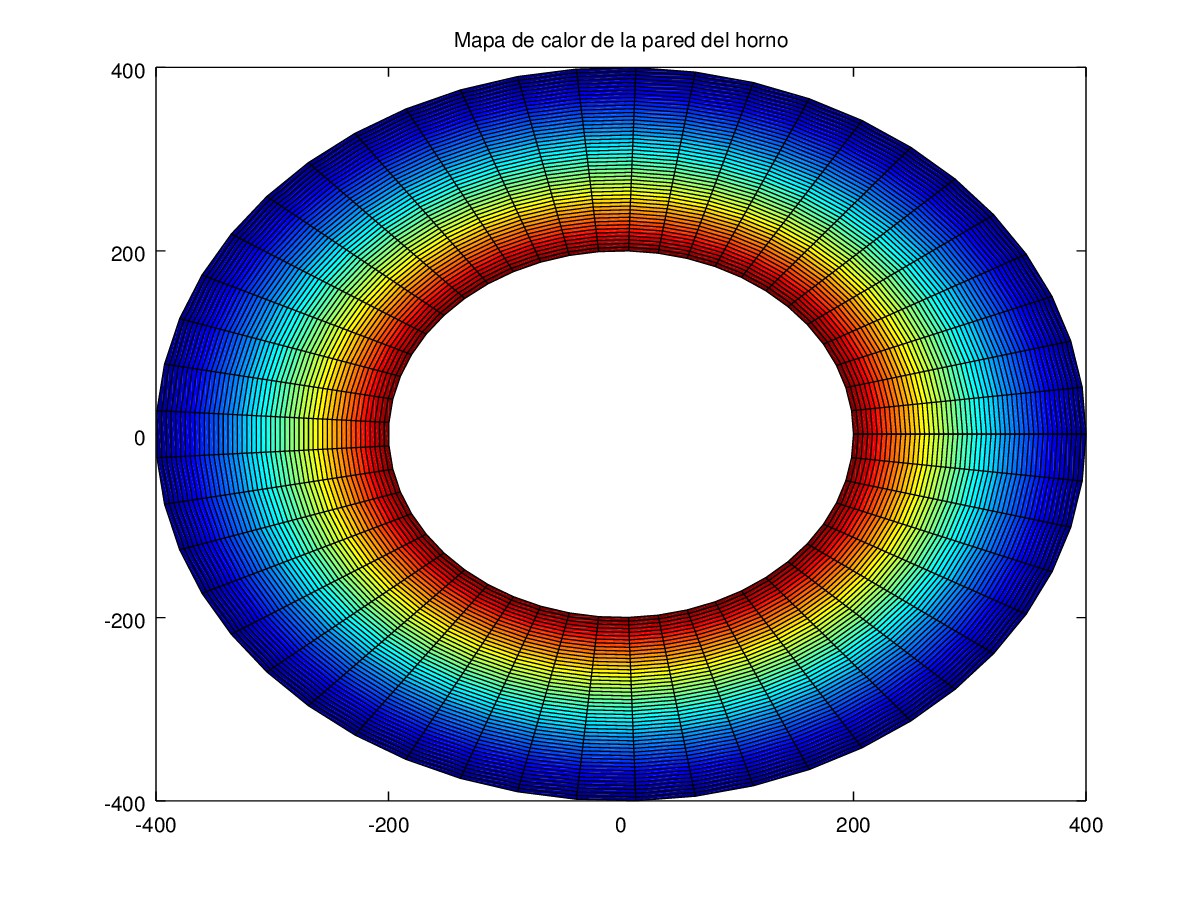
\includegraphics[scale=0.35]{experimentos1a_1b/evolucion_posicion_isoterma_temperatura/variacion_angulos_radio_fijo_se_suaviza_isoterma/test10_050_radios_049_angulos_inst_001_heatmap.png}
		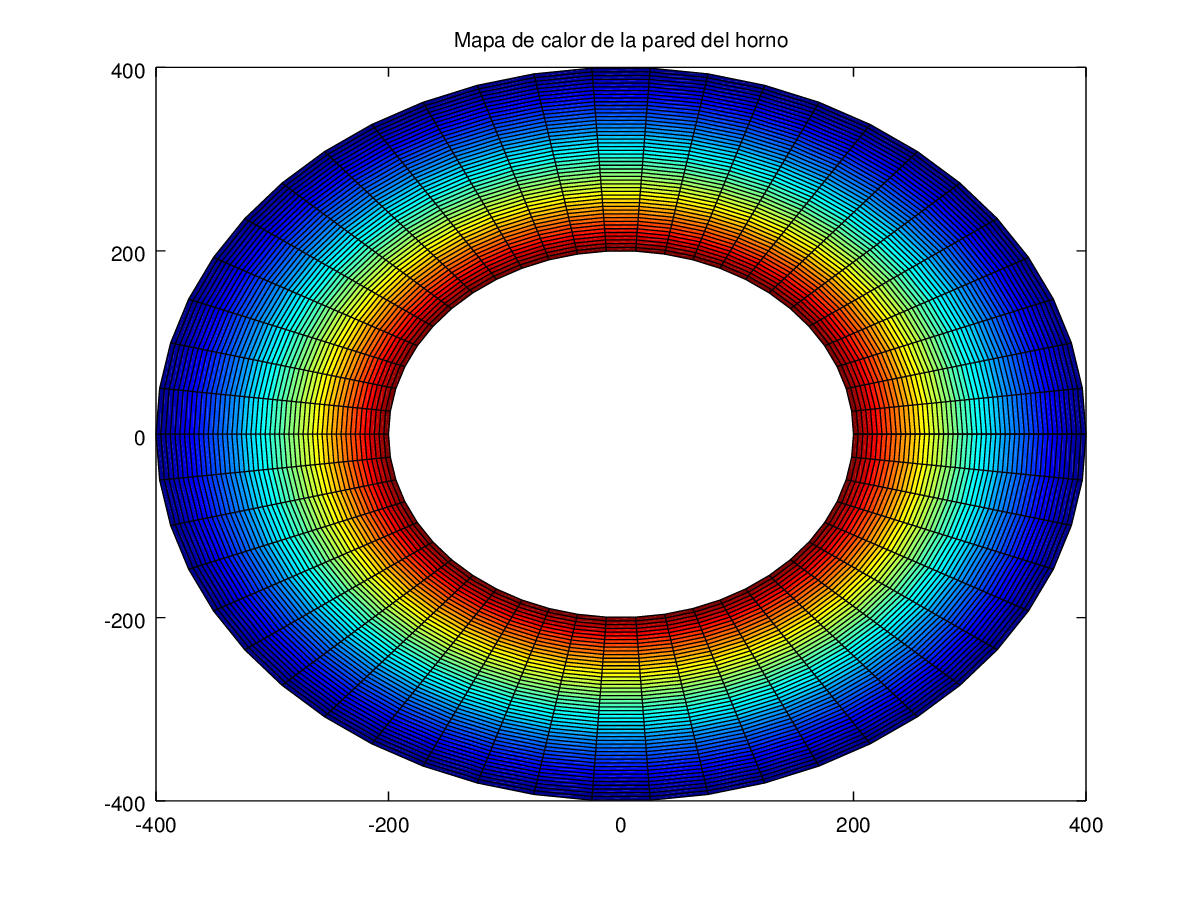
\includegraphics[scale=0.35]{experimentos1a_1b/evolucion_posicion_isoterma_temperatura/variacion_angulos_radio_fijo_se_suaviza_isoterma/test10_050_radios_050_angulos_inst_001_heatmap.png}

\vspace{0.5cm}

Aquí el radio es el mismo, pero se gana en precisión al tener más ángulos por no tener que linealizar la posición de la isoterma angularmente. Nuevamente, la posición entre dos tests consecutivos se estabiliza al aumentar la cantidad de ángulos. Tambien se observa que al cambiar el $\Delta_\theta$ los ángulos entre tests consecutivos no son los mismos.

	\item \begin{itemize}
						\item \textbf{Temperaturas internas y externas:} constantes, 100 y 1500. Esto es para que tenga la misma solución cada test del experimento.
						\item \textbf{Radio interno:} 200
						\item \textbf{Radio externo:} 400
						\item \textbf{Cantidad radios:} $[15\dots60]$
						\item \textbf{Cantidad ángulos:} $[15\dots60]$
						\item \textbf{Isoterma buscada:} 500
					\end{itemize}
	Se adjunta con el trabajo práctico un video que expone la evolución del sistema mientras se incrementa la cantidad de radios. Expondremos estáticamente algunos frames, pero es conveniente ver el video primero. Se encuentra en la misma carpeta que el pdf. (variación\_doble\_isomap.mp4, variación\_doble\_heatmap.mp4).

	\vspace{0.5cm}
	  	\textbf{Variación de la estimación de la isoterma entre 15 y 16 radios, ángulos de discretización}\\
		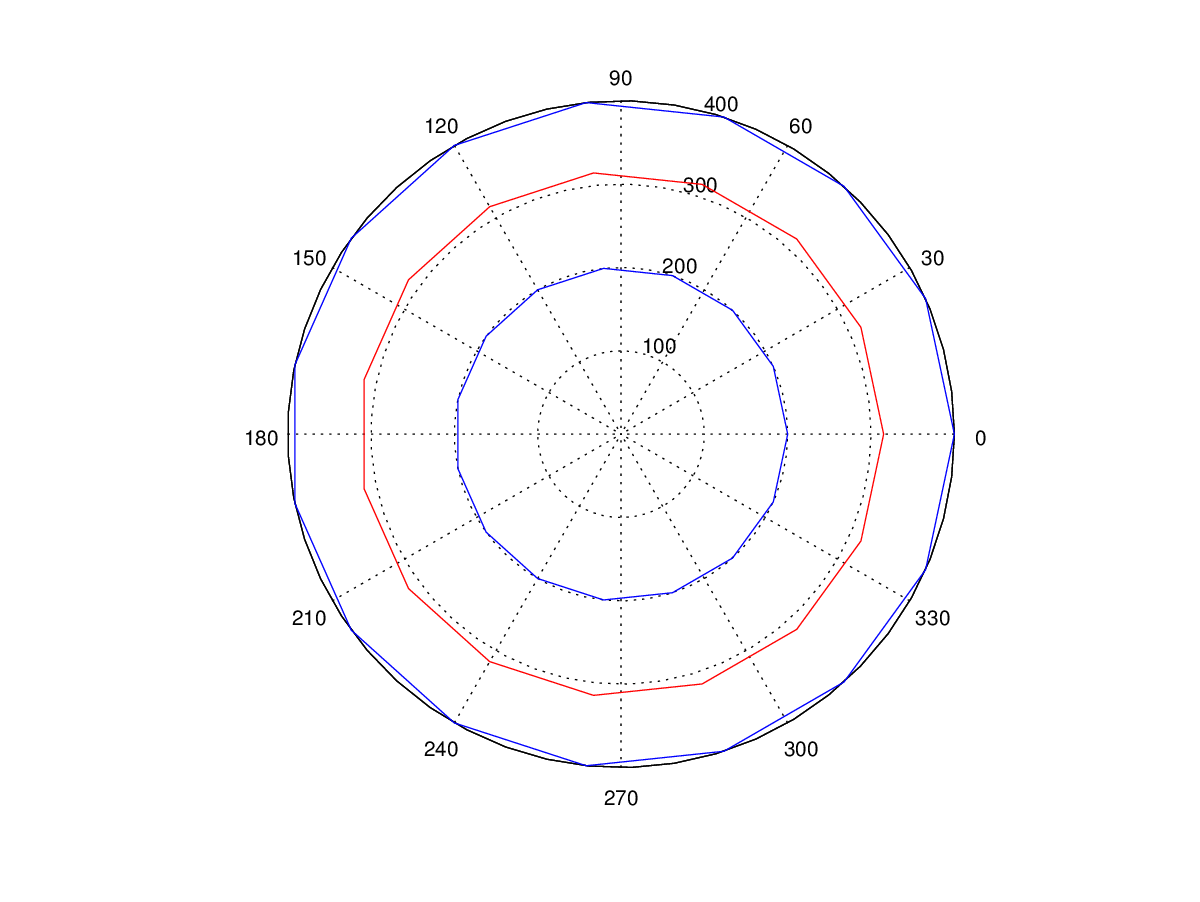
\includegraphics[scale=0.35]{experimentos1a_1b/evolucion_posicion_isoterma_temperatura/variacion_radios_angulos_se_reduce_diferencia_radial/test11_testord_001_inst_001_isomap.png}
		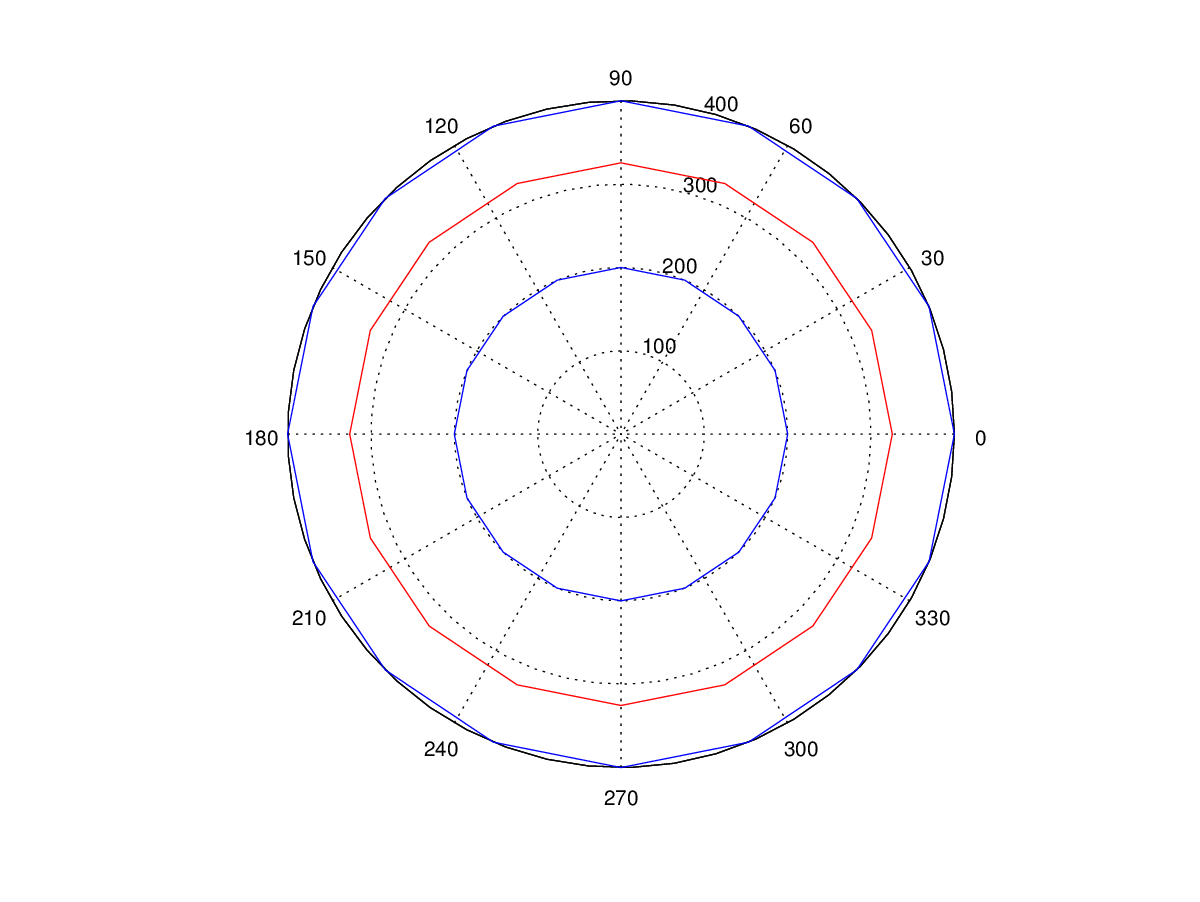
\includegraphics[scale=0.35]{experimentos1a_1b/evolucion_posicion_isoterma_temperatura/variacion_radios_angulos_se_reduce_diferencia_radial/test11_testord_002_inst_001_isomap.png}

	  	\textbf{Variación de la temperatura entre 59 y 60 radios, ángulos de discretización}\\
	  	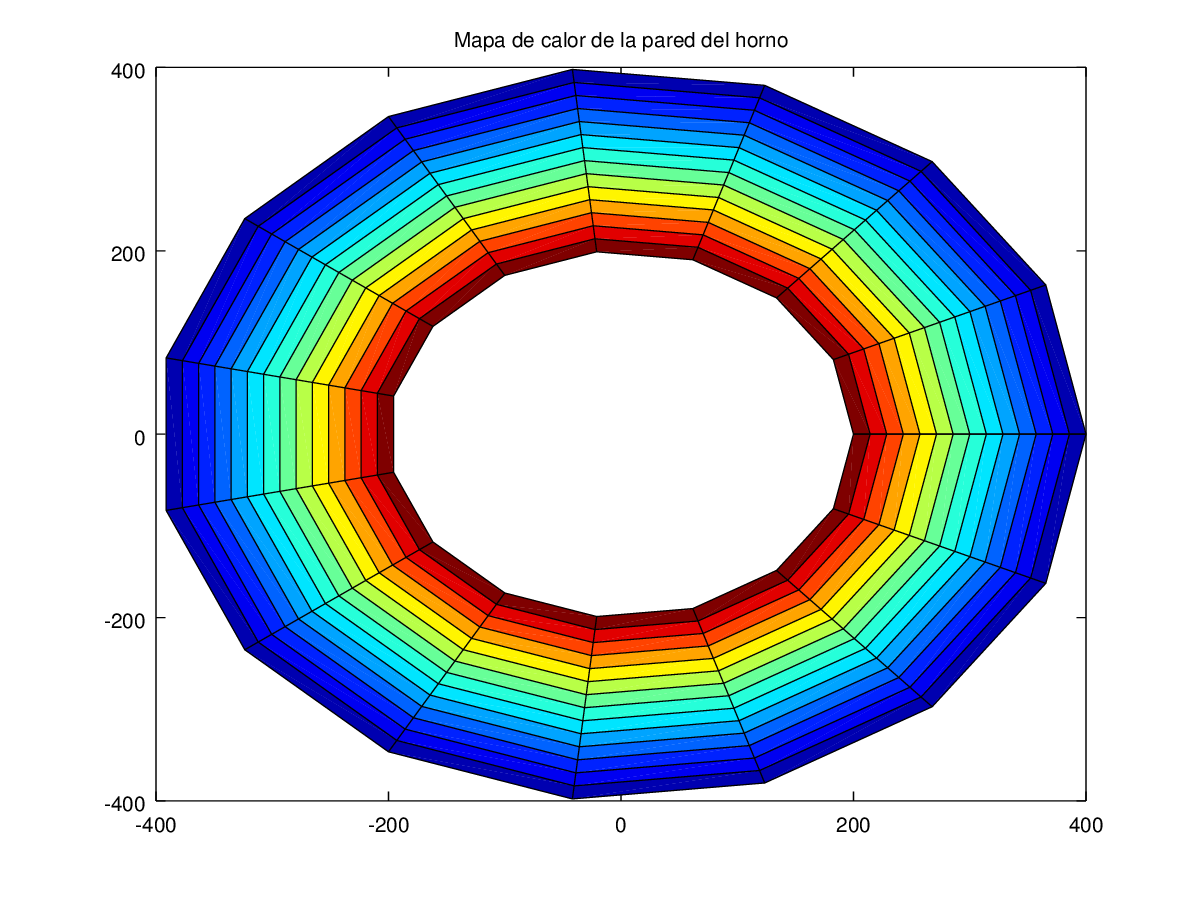
\includegraphics[scale=0.35]{experimentos1a_1b/evolucion_posicion_isoterma_temperatura/variacion_radios_angulos_se_reduce_diferencia_radial/test11_testord_001_inst_001_heatmap.png}
		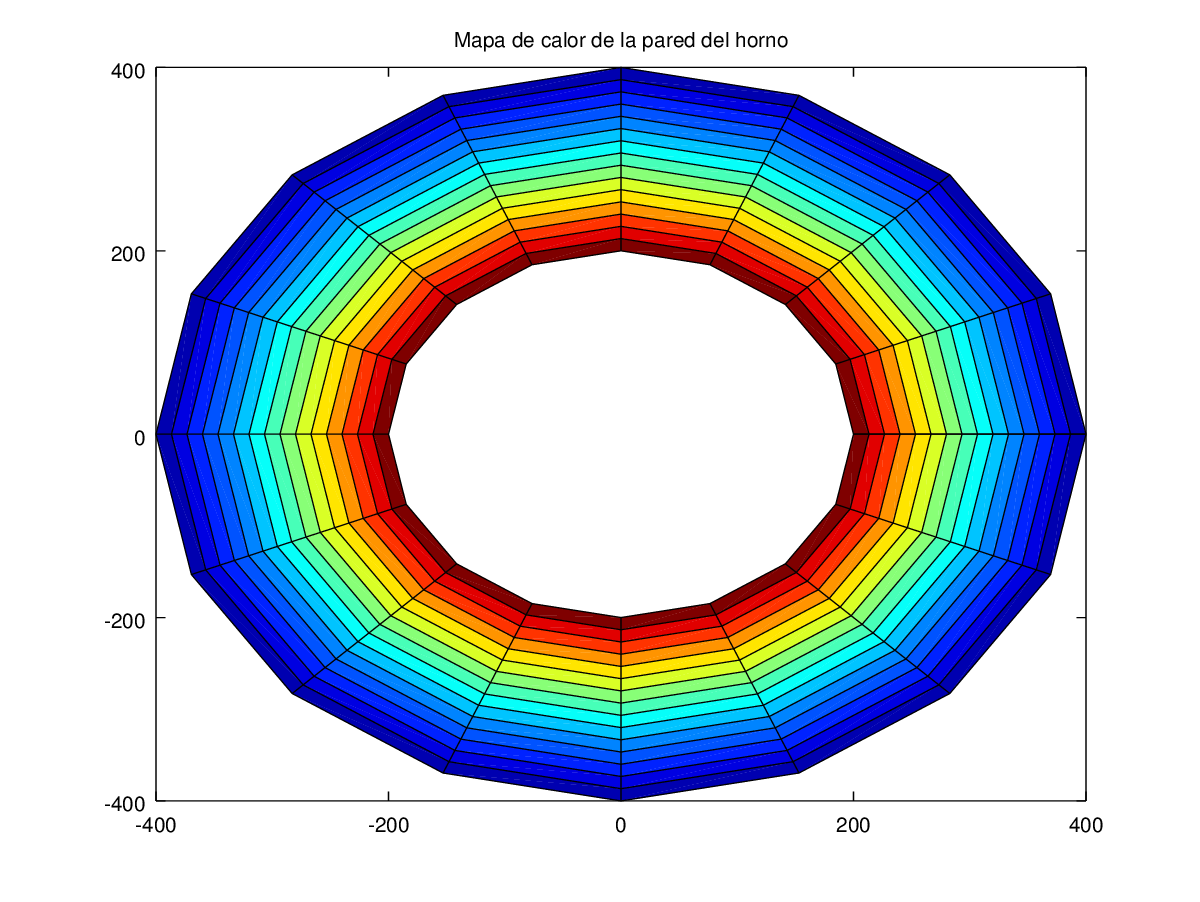
\includegraphics[scale=0.35]{experimentos1a_1b/evolucion_posicion_isoterma_temperatura/variacion_radios_angulos_se_reduce_diferencia_radial/test11_testord_002_inst_001_heatmap.png}

	  	\textbf{Variación de la estimación de la isoterma entre 15 y 16 radios, ángulos de discretización}\\
		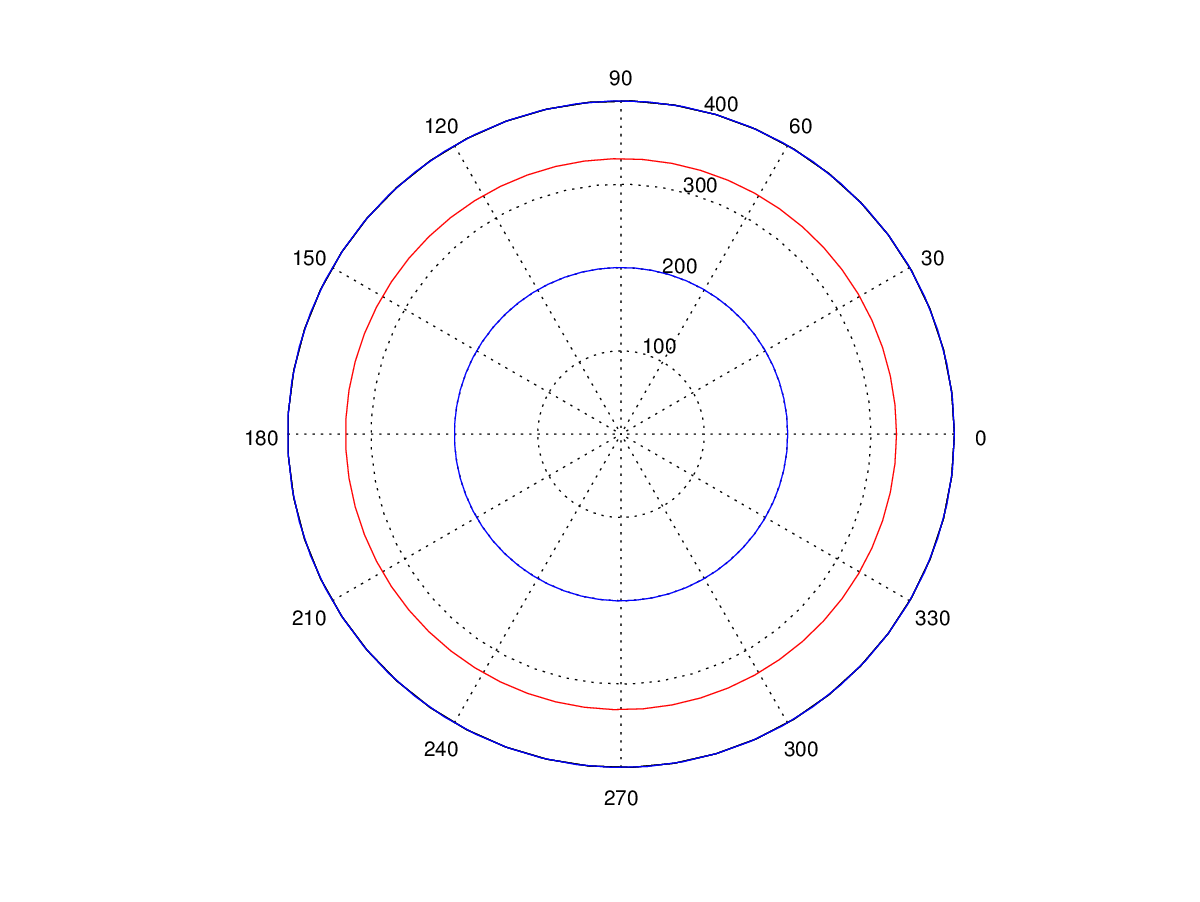
\includegraphics[scale=0.35]{experimentos1a_1b/evolucion_posicion_isoterma_temperatura/variacion_radios_angulos_se_reduce_diferencia_radial/test11_testord_045_inst_001_isomap.png}
		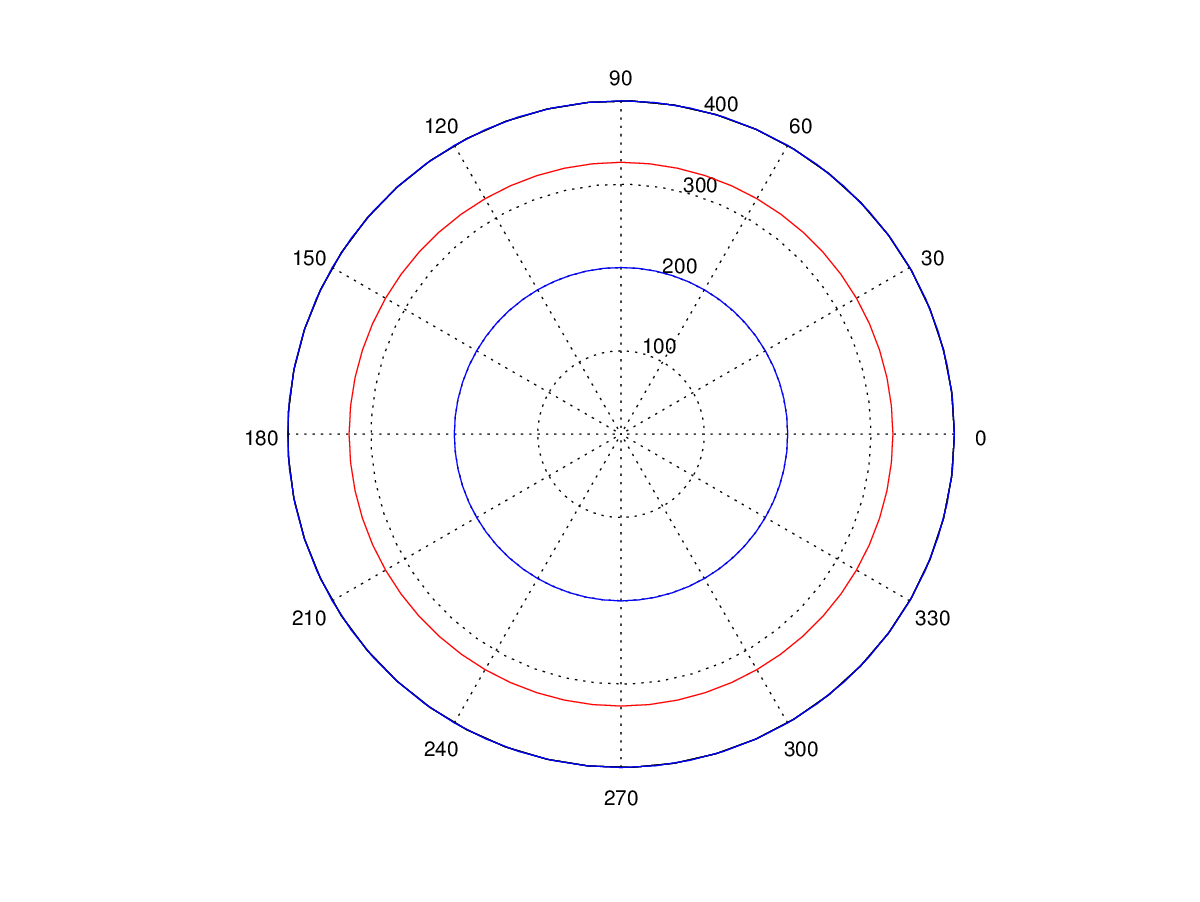
\includegraphics[scale=0.35]{experimentos1a_1b/evolucion_posicion_isoterma_temperatura/variacion_radios_angulos_se_reduce_diferencia_radial/test11_testord_046_inst_001_isomap.png}

		\textbf{Variación de la temperatura entre 59 y 60 radios, ángulos de discretización}\\
	  	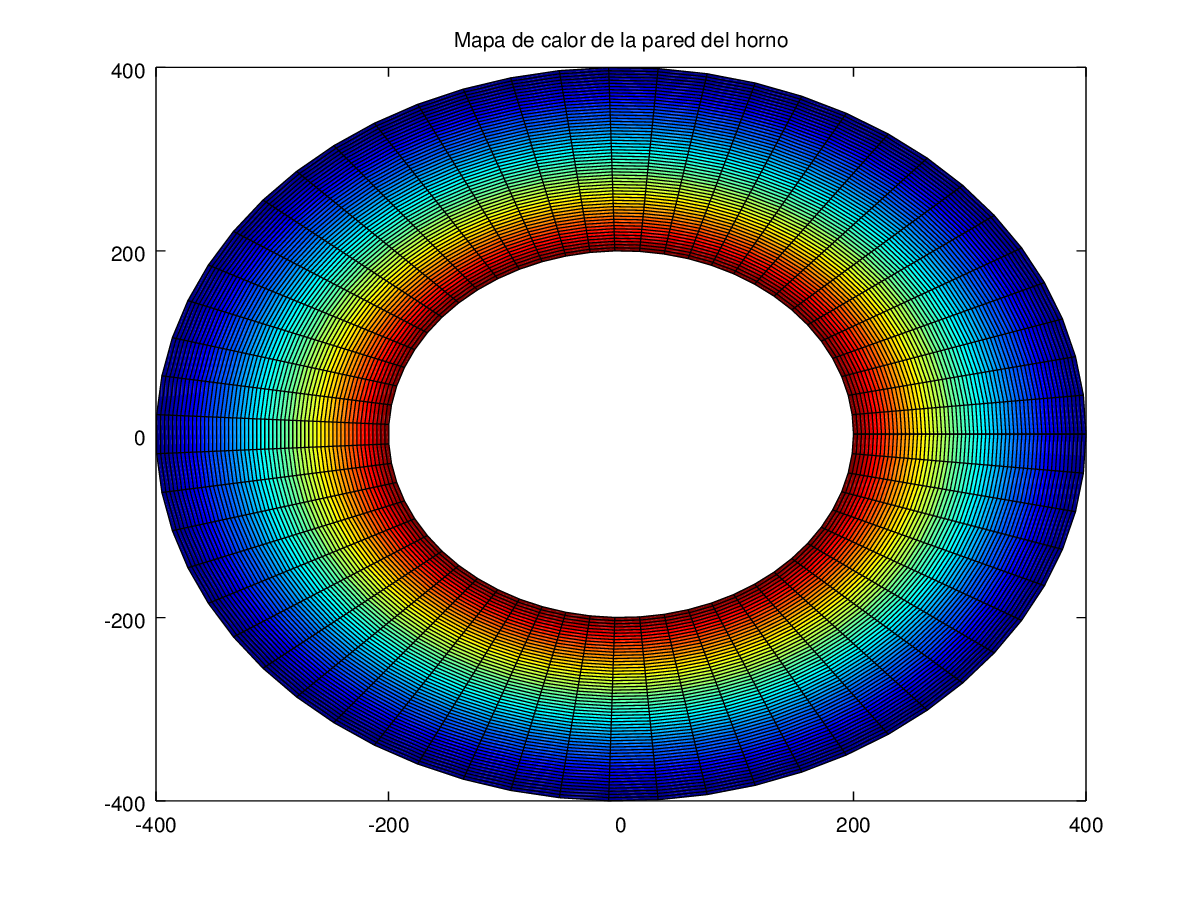
\includegraphics[scale=0.35]{experimentos1a_1b/evolucion_posicion_isoterma_temperatura/variacion_radios_angulos_se_reduce_diferencia_radial/test11_testord_045_inst_001_heatmap.png}
		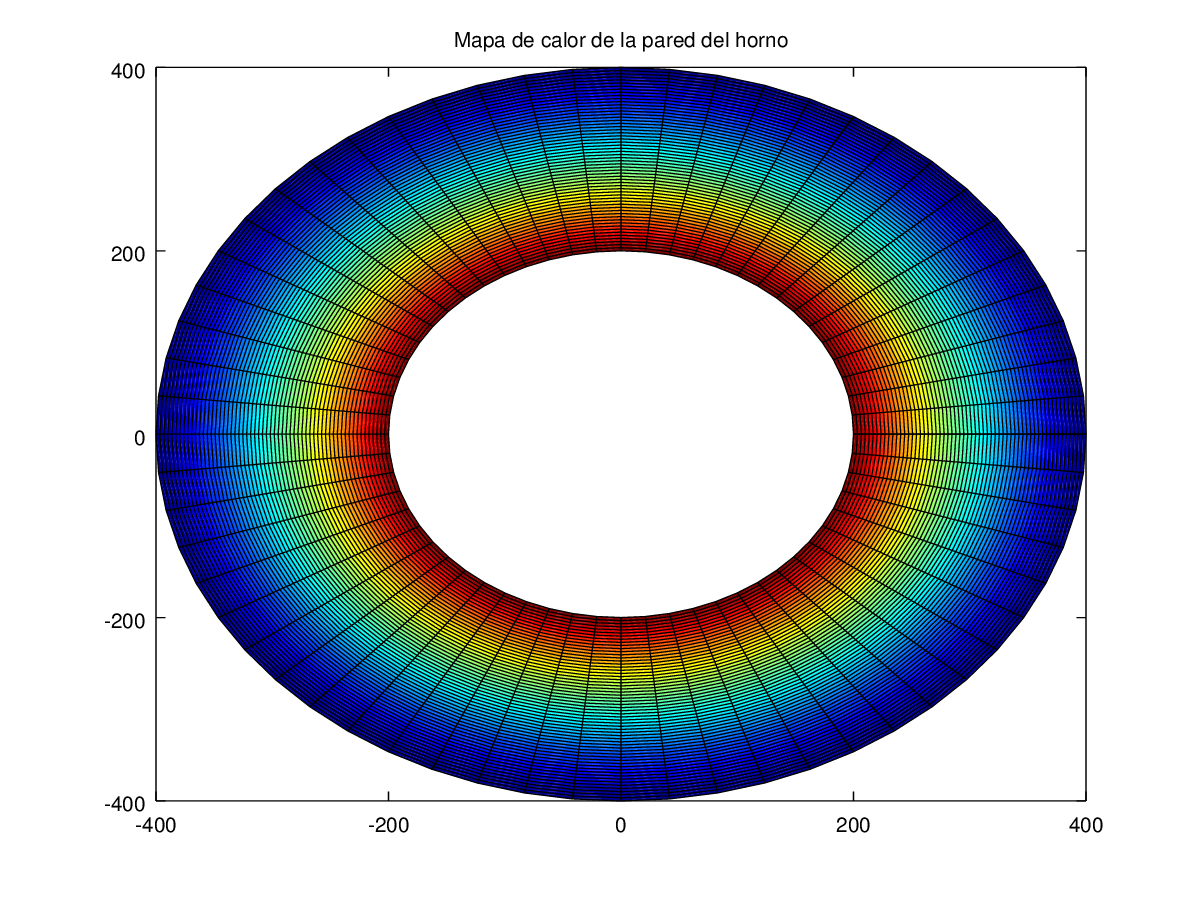
\includegraphics[scale=0.35]{experimentos1a_1b/evolucion_posicion_isoterma_temperatura/variacion_radios_angulos_se_reduce_diferencia_radial/test11_testord_046_inst_001_heatmap.png}
\FloatBarrier
\vspace{0.5cm}

En este último ejemplo ocurren ambos fenomenos al mismo tiempo, hay una variación radial menor a medida que crecen los radios y la curva se suaviza al aumentar los ángulos.

\end{enumerate}

\vspace{0.5cm}

Efectivamente, podemos concluir que mientras más fina sea la discretización, se obtendrán resultados más \texttt{estables y confiables} acerca de la estimación. Uno de los motivos es porque habrá menos puntos para interpolar en la posición de la isoterma y el otro porque se tiene más informacion de la temperatura de la pared del horno.

\subsubsection{Estimación de estabilidad de la pared del horno}

Se presentarán a continuación los resultados de la estimacion de la estabilidad del horno. Para varios tipos de discretizaciones donde la cantidad de ángulos y radios son iguales, se evalua el cambio de posicion de la isoterma a medida que va aumentando la temperatura externa entre 100 y 300 grados, de a 2 grados por paso. Dado que las temperaturas son constantes, el máximo y el promedio coinciden como métricas de posicionamiento relativo de la isoterma.

\begin{figure}[h]
\centering

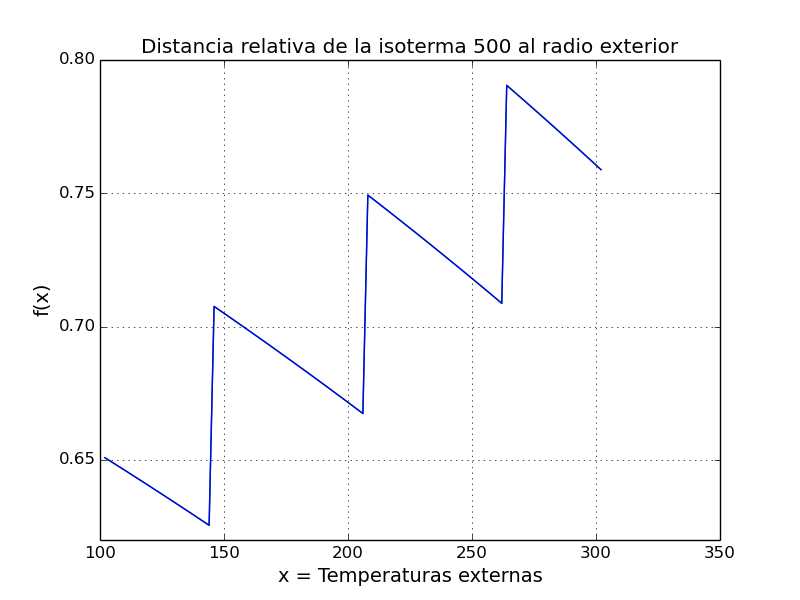
\includegraphics[scale=0.3]{experimentos1a_1b/evolucion_estimacion_seguridad_isoterma/variacion_25.png}
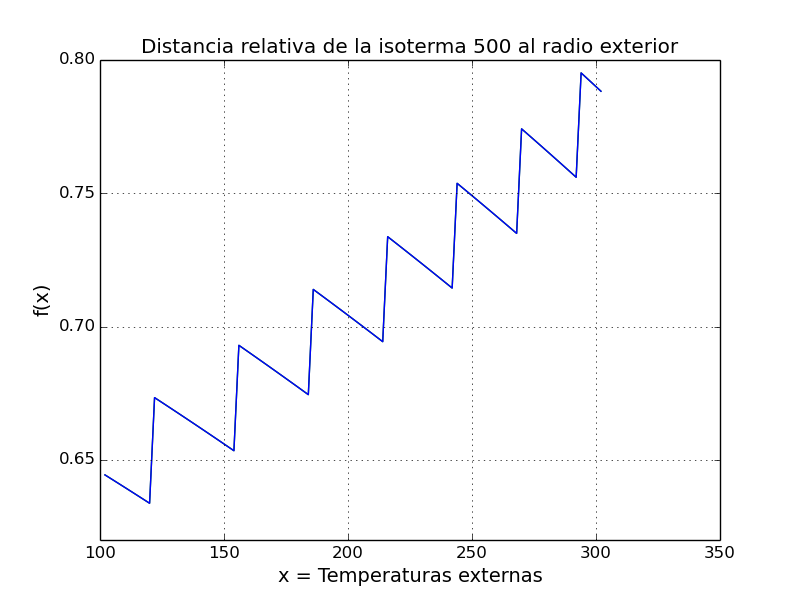
\includegraphics[scale=0.3]{experimentos1a_1b/evolucion_estimacion_seguridad_isoterma/variacion_50.png}	

\caption{Cantidad de radios y ángulos: 25(Izq) 50(Der)}
\end{figure}

\begin{figure}[h]
\centering

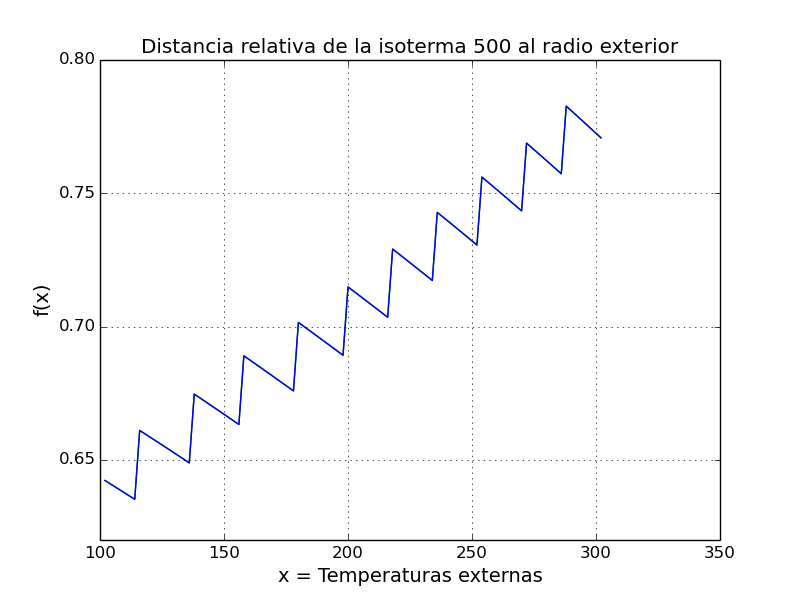
\includegraphics[scale=0.3]{experimentos1a_1b/evolucion_estimacion_seguridad_isoterma/variacion_75.png}
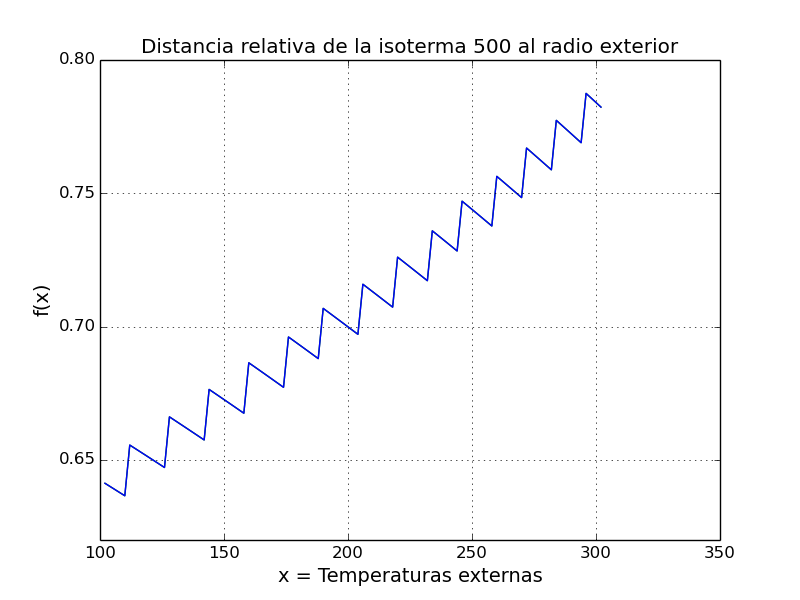
\includegraphics[scale=0.3]{experimentos1a_1b/evolucion_estimacion_seguridad_isoterma/variacion_100.png}	

\caption{Cantidad de radios y ángulos: 75(Izq) 100(Der)}
\end{figure}

\begin{figure}[h]
\centering

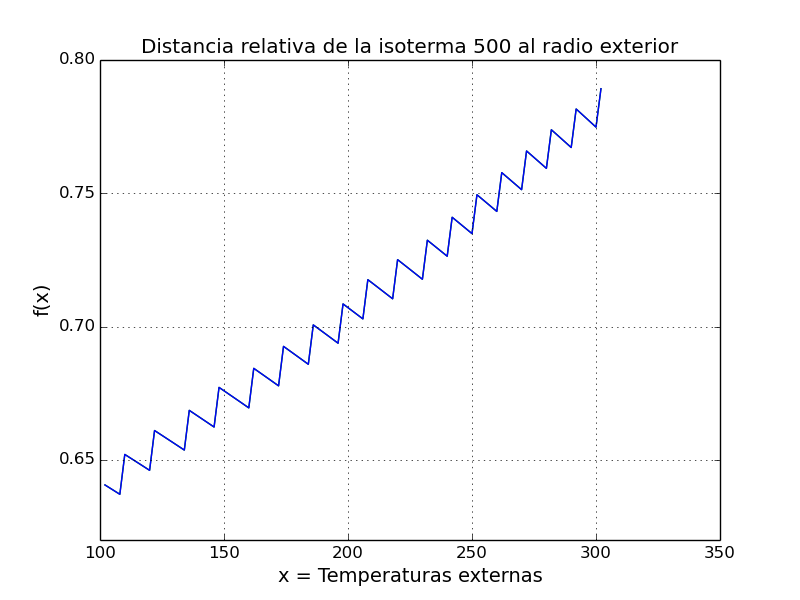
\includegraphics[scale=0.5]{experimentos1a_1b/evolucion_estimacion_seguridad_isoterma/variacion_125.png}

\caption{Cantidad de radios y ángulos: 125}
\end{figure}

\begin{figure}[h]
\centering

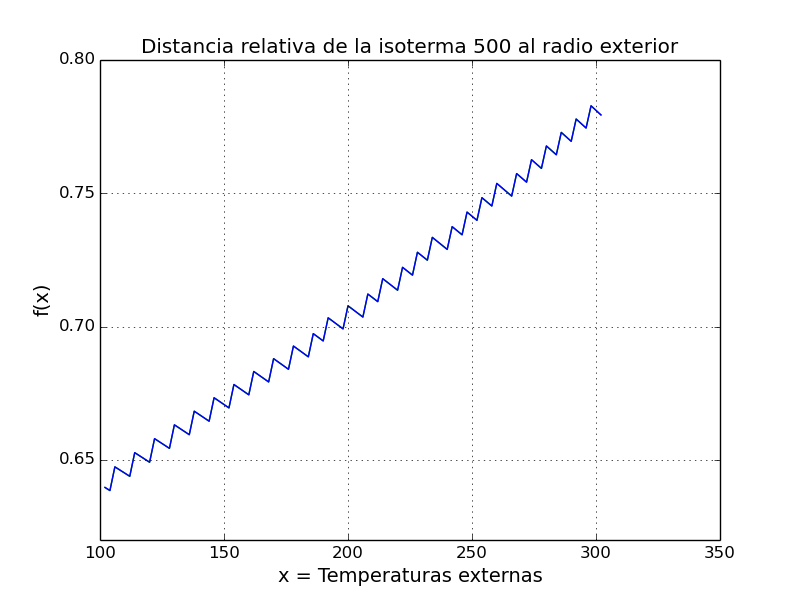
\includegraphics[scale=0.5]{experimentos1a_1b/evolucion_estimacion_seguridad_isoterma/variacion_30a_200r.png}
\caption{Cantidad de radios 200 - ángulos: 30}

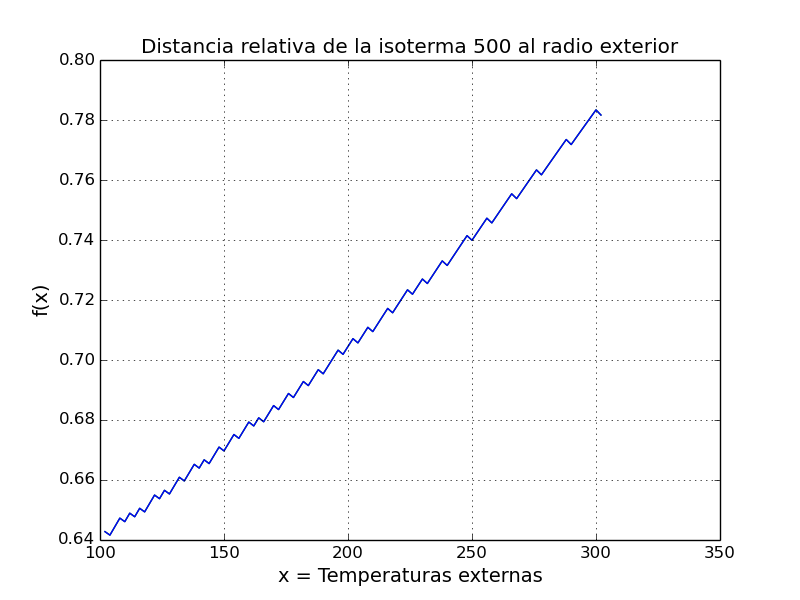
\includegraphics[scale=0.5]{experimentos1a_1b/evolucion_estimacion_seguridad_isoterma/variacion_5a_500r.png}
\caption{Cantidad de radios 500 - ángulos: 5}
\end{figure}
\FloatBarrier

Los gráficos son un poco mas extraños de lo esperado. Se observa que, para cualquier discretizacion fija, al aumentar la temperatura externa, la isoterma tiende a acercarse a la pared externa. Esto es lo esperable, el método propuesto para determinar la seguridad de la isoterma consiste en fijar un umbral sobre la posicion relativa máxima o promedio. Lo que se observa como raro es la curva \texttt{dentada} a medida que crecen las temperaturas. Veamos además que estos \texttt{dientes} disminuyen su intensidad a medida que se van agregando radios a la discretizacion. 

\begin{proposition} 
	Bajo que las temperaturas internas y externas constantes, la posicion radial de la isoterma es la misma en todo ángulo.	
\end{proposition}

Dada esta última proposición, podemos hacer experimentos con muy pocos ángulos y muchos radios que nos den pauta de que ocurre con esos \texttt{dientes} en los gráficos. \\
Se puede observar en las figuras con 200 y 500 radios, que a medida que $m\to\infty$ , la curva se suaviza. Lo cual nos hace pensar, que la estimacion lineal de la isoterma esta generando esta distorsión.

\vspace{0.5cm}

Consideremos nuevamente $\hat{g_{\theta_i}}$: la función \textbf{discreta de aproximaciones} de temperatura de un ángulo i. A medida que las temperaturas aumentan linealmente, los 2 puntos $x$ y $x'$ que acotan la isoterma buscada en dicha función van aumentando tambien, generando que la estimacion del punto intermedio entre ellos decrezca. Creemos que cuando esos 2 puntos dejan se encerrar el valor buscado, es que se produce el \texttt{salto} en el gráfico.

\begin{proposition}
	El método de umbral de seguridad es inconsistente tomando la distancia máxima relativa o distancia promedio relativa a la pared exterior.
\end{proposition}

En los resultados anteriores y en el gráfico presentado en el primer experimento de ubicacion de la isoterma (convergencia radial de la isoterma). Se puede observar claramente, que trazando una recta horizontal en algún punto del eje Y, la determinación de colapso no es consistente. Es decir, existen $t_1 < t_2 < t_3$ temperaturas crecientes donde tanto la posicion máxima relativa o la posicion promedio relativa, indican peligro de colapso para $t_2$ pero no para $t_1$ ni $t_3$. Sin embargo, cuando $m\to\infty$ esto tiende a ser \texttt{menos inconsistente}.

\subsubsection{Análisis de la interpolacion lineal de la curva de temperatura}

Dados los resultados de la sección anterior, nos interesó saber un poco mas la forma de la funcion de temperatura sobre un ángulo fijo $\hat{g_{\theta_i}}$. 
Variamos un poco la cantidad de radios, y graficamos la función obtenida de los puntos de la discretización en una dirección fija y un fitteo lineal.
El resultado de los gráficos muestra que la temperatura no se disipa linealmente entre el interior y el exterior del horno. Dado que nosotros aproximamos linealmente la posicion radial de la isoterma 500 \textbf{entre los 2 puntos mas cercanos}, tendremos un error en cada \texttt{cambio de puntos} para la aproximacion.\\

Esto fortalece nuestra hipótesis de la sección anterior de que la forma de diente de sierra de los gráficos podía deberse a la interpolacion de algo no lineal, mediante una recta en puntos consecutivos.

\begin{figure}[h]
\centering
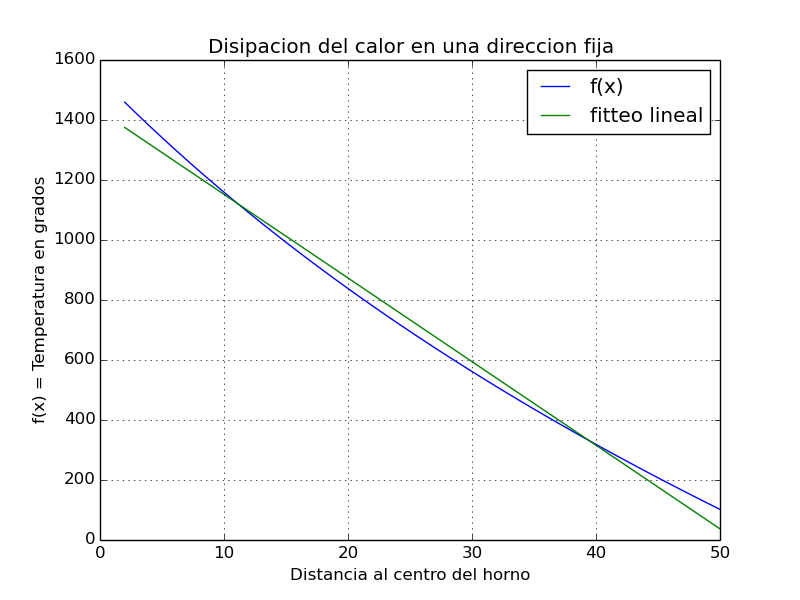
\includegraphics[scale=0.34]{funcion_temp_50_radios_ti_1500_te_102.png}
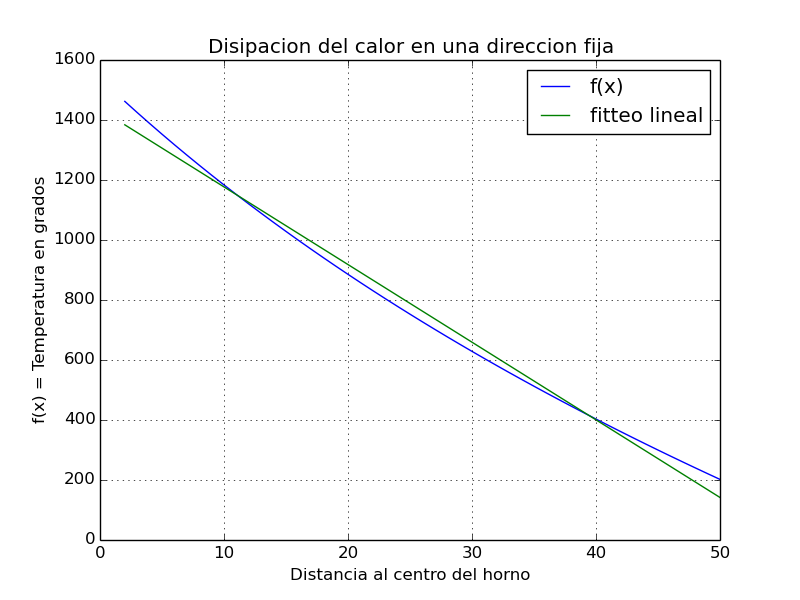
\includegraphics[scale=0.34]{funcion_temp_50_radios_ti_1500_te_202.png}
\caption{Distintas temperaturas externas - Cantidad de radios: 50}
\end{figure}
\FloatBarrier

\begin{figure}[h]
\centering
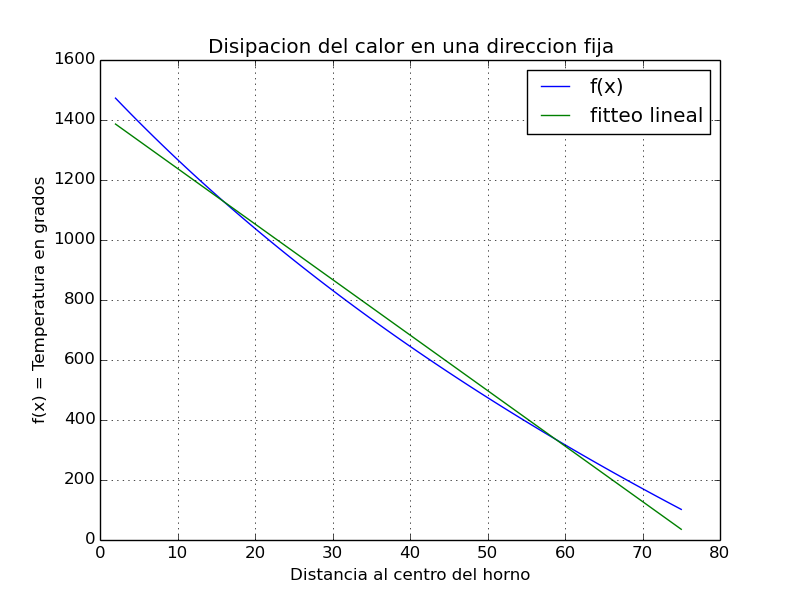
\includegraphics[scale=0.34]{funcion_temp_75_radios_ti_1500_te_102.png}
\includegraphics[scale=0.34]{funcion_temp_75_radios_ti_1500_te_202.png}
\caption{Distintas temperaturas externas - Cantidad de radios: 75}
\end{figure}
\FloatBarrier

\begin{figure}[h]
\centering
\includegraphics[scale=0.34]{funcion_temp_150_radios_ti_1500_te_102.png}
\includegraphics[scale=0.34]{funcion_temp_500_radios_ti_1500_te_102.png}
\caption{Cantidad de radios: 150(izq) , 500(der)}
\end{figure}
\FloatBarrier

\begin{figure}[h]
\centering
\includegraphics[scale=0.8]{efecto_interpolacion_lineal.png}
\caption{Esquema aproximado: Efecto interpolacion lineal entre puntos de algo no lineal}
\label{fig:aprox}
\end{figure}
\FloatBarrier

En la figura \ref{fig:aprox} se ve lo que podría estar ocurriendo al aproximar linealmente 2 puntos de una curva que realmente no es lineal. La recta entre dos puntos queda por encima de la curva real, luego, si se quiere hallar el $x$ tal que $g(x) = \alpha$ , la aproximación falla por un $\epsilon$ que depende de la concavidad de la curva respecto a la recta. A medida que se van agregando radios a la discretizacion, la distancia entre los puntos que se aproximan disminuye, disminuyendo el error cometido al estimar. 


\clearpage

\section{Discusión}
% TODO
Se incluira aqu un analisis de los resultados obtenidos en la seccion anterior (se analizara
su  validez,  coherencia,  etc.).   Deben  analizarse  como  mnimo  los tems  pedidos  en  el
enunciado.  No es aceptable decir que los resultados fueron los esperados", sin hacer
clara referencia a la teora a la cual se ajustan.  Ademas, se deben mencionar los resul-
tados interesantes y los casos patologicos" encontrados.


\clearpage

\section{Conclusiones}
%!TEX root = informe.tex
\IEEEPARstart{A}{} lo largo de este trabajo atacamos el problema de generar frames artificiales para un video, intentando lograr que se ajusten al original hasta el punto -ideal- de que el ojo humano no detecte la diferencia con un video filmado en alta frecuencia.

Como primera conclusión al respecto podemos decir que no logramos dicho objetivo ideal: de nuestras observaciones descubrimos fácilmente que, al menos para los tres métodos implementados, los resultados ``no engañan a nadie''. Todos los métodos presentan o bien \emph{lag} o bien \emph{fantasmeo}, perturbando la sensación de fluidez y alterando el realismo percibido del video.

Más allá de ese análisis cualitativo, pudimos observar que atacar el problema de forma \emph{naïve} (el método que llamamos ``Vecino más cercano'') produce resultados con error matemático más reducido aunque visualmente pareciera ser el peor método, pudiendo obtenerse resultados visualmente más agradables con métodos más inteligentes como interpolación mediante poliniomios.

También concluimos que, visto como método de compresión, los resultados son pobres. En la actualidad existen métodos que, sin utilizar mucho más espacio, generan prácticamente nulos \emph{artifacts} y no pierden información de cuadros completos.

\section{Apéndice}
\subsection{Apéndice A: Enunciado}
% 
\begin{centering}
\bf Laboratorio de M\'etodos Num\'ericos - Segundo Cuatrimestre 2015 \\
\bf Trabajo Pr\'actico N\'umero 1: Con 15 $\theta$s discretizo alto horno\ldots\\
\end{centering}

\vskip 25pt
\hrule
\vskip 11pt

{\bf Introducción}

Consideremos la secci\'on horizontal de un horno de acero cil\'indrico, como en la Figura 1. El sector A es la pared del horno, y el sector B es el horno propiamente dicho, en el cual se funde el acero a temperaturas elevadas. Tanto el borde externo como el borde interno de la pared forman c\'irculos. Suponemos que la temperatura del acero dentro del horno (o sea, dentro de B) es constante e igual a 1500$^{o}$C.

\medskip

Tenemos sensores ubicados en la parte externa del horno para medir la temperatura de la pared externa del mismo, que habitualmente se encuentra entre 50$^{o}$C y 200$^{o}$C. El problema que debemos resolver consiste en estimar la isoterma de 500$^{o}$C dentro de la pared del horno, para estimar la resistencia de la misma. Si esta isoterma est\'a demasiado cerca de la pared externa del horno, existe peligro de que la estructura externa de la pared colapse.


\begin{figure}[ht]
\begin{center}
\includegraphics[width=0.6\columnwidth]{img/Horno.png}
\caption{Secci\'on circular del horno}
\end{center}
\end{figure}



El objetivo del trabajo práctico es implementar un programa que calcule la isoterma solicitada, conociendo las dimensiones del horno y las mediciones de temperatura en la pared exterior.

{\bf El Modelo}

Sea $r_e \in \mathbb{R}$ el radio exterior de la pared y sea $r_i \in \mathbb{R}$ el radio interior de la pared. Llamemos $T(r,\theta)$ a la temperatura en el punto dado por las coordenadas polares $(r,\theta)$, siendo $r$ el radio y $\theta$ el \'angulo polar de dicho punto. En el estado estacionario, esta temperatura satisface la ecuaci\'on del calor:

\begin{equation}\label{calor}
\frac{\partial^2T(r,\theta)}{\partial r^2}+\frac{1}{r}\frac{\partial T(r,\theta)}{\partial r}+\frac{1}{r^2}\frac{\partial^2T(r,\theta)}{\partial \theta^2} = 0 
\end{equation}


Si llamamos $T_i \in \mathbb{R}$ a la temperatura en el interior del horno (sector B) y $T_e : [0,2\pi] \rightarrow \mathbb{R}$ a la funci\'on de temperatura en el borde exterior del horno (de modo tal que el punto $(r_e,\theta)$ tiene temperatura $T_e(\theta)$), entonces tenemos que

\begin{equation}
T(r,\theta) = T_i \;\;\;\;\;para\;todo\;punto\;(r,\theta)\;con\;r\leq r_i
\end{equation}
\begin{equation}
T(r_e,\theta) = T_e(\theta) \;\;\;\;\;\;para\;todo\;punto\;(r_e,\theta)
\end{equation}


El problema en derivadas parciales dado por la primera ecuaci\'on con las condiciones de contorno presentadas recientemente, permite encontrar la funci\'on $T$ de temperatura en el interior del horno (sector A), en funci\'on de los datos mencionados en esta secci\'on.

Para resolver este problema computacionalmente, discretizamos el dominio del problema (el sector A) en coordenadas polares. Consideramos una partici\'on $0 = \theta_0 < \theta_1 < ... < \theta_n = 2\pi$ en $n$ \'angulos discretos con $\theta_k-\theta_{k-1} = \Delta\theta$ para $k = 1,...,n$, y una partici\'on $r_i = r_0 < r_1 < ... < r_m = r_e$ en $m+1$ radios discretos con $r_j - r_{j-1} = \Delta r$ para $j = 1,...,m$.

\medskip

El problema ahora consiste en determinar el valor de la funci\'on $T$ en los puntos de la discretizaci\'on $(r_j,\theta_k)$ que se encuentren dentro del sector A. Llamemos $t_{jk} = T(r_j,\theta_k)$ al valor (desconocido) de la funci\'on $T$ en el punto $(r_j,\theta_k)$.

\medskip

Para encontrar estos valores, transformamos la ecuaci\'on (\ref{calor}) en un conjunto de ecuaciones lineales sobre las inc\'ognitas $t_{jk}$, evaluando (\ref{calor}) en todos los puntos de la discretizaci\'on que se encuentren dentro del sector A. Al hacer esta evaluaci\'on, aproximamos las derivadas parciales de $T$ en (\ref{calor}) por medio de las siguientes f\'ormulas de diferencias finitas:


\begin{equation}
\frac{\partial^2T(r,\theta)}{\partial r^2}(r_j,\theta_k) \cong \frac{t_{j-1,k}-2t_{jk}+t_{j+1,k}}{(\Delta r)^2}
\end{equation}

\begin{equation}
\frac{\partial T(r,\theta)}{\partial r}(r_j,\theta_k) \cong \frac{t_{j,k}-t_{j-1,k}}{\Delta r}
\end{equation}

\begin{equation}
\frac{\partial^2T(r,\theta)}{\partial \theta^2}(r_j,\theta_k) \cong \frac{t_{j,k-1}-2t_{jk}+t_{j,k+1}}{(\Delta \theta)^2}
\end{equation}



Es importante notar que los valores de las inc\'ognitas son conocidos para los puntos que se encuentran sobre el borde exterior de la pared, y para los puntos que se encuentren dentro del sector B. Al realizar este procedimiento, obtenemos un sistema de ecuaciones lineales que modela el problema discretizado. La resoluci\'on de este sistema permite obtener una aproximaci\'on de los valores de la funci\'on $T$ en los puntos de la discretizaci\'on.

{\bf Enunciado}

Se debe implementar un programa en \verb+C+ o \verb-C++- que tome como entrada los par\'ametros del problema ($r_i$, $r_e$, $m+1$,
$n$, valor de la isoterma buscada, $T_i$, $T_e(\theta)$) que calcule la temperatura dentro de la pared del horno utilizando el
modelo propuesto en la secci\'on anterior y que encuentre la isoterma buscada en funci\'on del resultado obtenido del
sistema de ecuaciones. El m\'etodo para determinar la posici\'on de la isoterma queda a libre elecci\'on de cada grupo y
debe ser explicado en detalle en el informe.

El programa debe formular el sistema obtenido a partir de las ecuaciones (1) - (6) y considerar dos m\'etodos posibles
para su resoluci\'on: mediante el algoritmo cl\'asico de Eliminaci\'on Gaussiana y la Factorizaci\'on LU. Finalmente, el
programa escribir\'a en un archivo la soluci\'on obtenida con el formato especificado en la siguiente secci\'on.

Como ya se ha visto en la materia, no es posible aplicar los m\'etodos propuestos para la resoluci\'on a cualquier
sistema de ecuaciones. Sin embargo, la matriz del sistema considerado en el presente trabajo cumple con ser diagonal dominante (no
estricto) y que, ordenando las variables y ecuaciones convenientemente, es posible armar un sistema de ecuaciones cuya matriz
posee la propiedad de ser \emph{banda}. Luego, se pide demostrar (o al menos dar un esquema de la demostraci\'on)
el siguiente resultado e incluirlo en el informe:

\begin{proposition}
Sea $A \in \mathbb{R}^{n \times n}$ la matriz obtenida para el sistema definido por (1)-(6). Demostrar que es posible
aplicar Eliminaci\'on Gaussiana sin pivoteo.\footnote{Sugerencia: Notar que la matriz es diagonal dominante (no
estrictamente) y analizar qué sucede al aplicar un paso de Eliminaci\'on Gaussiana con los elementos de una fila.} 
\end{proposition}

La soluci\'on del sistema de ecuaciones permitir\'a saber la temperatura en los puntos de la discretizaci\'on. Sin embargo,
nuestro inter\'es es calcular la isoterma 500, para poder determinar si la estructura se encuentra en peligro. Luego, se pide lo siguiente:
\begin{itemize}
\item Dada la soluci\'on del sistema de ecuaciones, proponer una forma de estimar en cada \'angulo de la discretizaci\'on la posici\'on de la 
isoterma 500.
\item En funci\'on de la aproximaci\'on de la isoterma, proponer una forma (o medida) a utilizar para evaluar la peligrosidad de la estructura
en funci\'on de la distancia a la pared externa del horno.
\end{itemize}


En funci\'on de la experimentaci\'on, se busca realizar dos estudios complementarios: por un lado, analizar c\'omo se comporta el sistema y, por otro, 
cu\'ales son los requerimientos computacionales de los m\'etodos. Se pide como m\'inimo realizar los siguientes experimentos:
\begin{enumerate}
\item Comportamiento del sistema.
\begin{itemize}
\item Considerar al menos dos instancias de prueba, generando distintas discretizaciones para cada una de ellas y
comparando la ubicaci\'on de la isoterma buscada respecto de la pared externa del horno. Se sugiere presentar gr\'aficos
de temperatura o curvas de nivel para los mismos, ya sea utilizando las herramientas provistas por la c\'atedra o
implementando sus propias herramientas de graficaci\'on. 
\item Estudiar la proximidad de la isoterma buscada respecto de la pared exterior del horno en funci\'on de distintas 
granularidades de discretizaci\'on y las condiciones de borde. 
\end{itemize}
\item Evaluaci\'on de los m\'etodos.
\begin{itemize}
\item Analizar el tiempo de c\'omputo requerido para obtener la soluci\'on del sistema en funci\'on de la granularidad de 
la discretizaci\'on. Se sugiere presentar los resultados mediante gr\'aficos de tiempo de c\'omputo en funci\'on de alguna 
de las variables del problema.
\item Considerar un escenario similar al propuesto en el experimento 1. pero donde las condiciones de borde (i.e., $T_i$ y $T_e(\theta)$)
cambian en distintos instantes de tiempo. En este caso, buscamos obtener la secuencia de estados de la temperatura en
la pared del horno, y la respectiva ubicaci\'on de la isoterma especificada. Para ello, se considera una secuencia de $ninst$
vectores con las condiciones de borde, y las temperaturas en cada estado es la soluci\'on del correspondiente sistema de
ecuaciones. Se pide formular al menos un experimento de este tipo, aplicar los m\'etodos de resoluci\'on propuestos de
forma conveniente y compararlos en t\'erminos de tiempo total de c\'omputo requerido para distintos valores de $ninst$.
\end{itemize}
\end{enumerate}

De manera opcional, aquellos grupos que quieran ir un poco m\'as all\'a pueden considerar trabajar y desarrollar alguno(s) 
de los siguientes puntos extra:
\begin{enumerate}
\item Notar que el sistema resultante tiene estructura \emph{banda}. Proponer una estructura para aprovechar este hecho en t\'erminos de la
\emph{complejidad espacial} y como se adaptar\'ian los algoritmos de Eliminaci\'on Gaussiana y Factorizaci\'on LU para reducir la
cantidad de operaciones a realizar.
\item Implementar dicha estructura y las adaptaciones necesarias para el algoritmo de Eliminaci\'on Gaussiana.
\item Implementar dicha estructura y las adaptaciones necesarias para el algoritmo de Factorizaci\'on LU. 
\end{enumerate}

Finalmente, se deber\'a presentar un informe que incluya una descripci\'on detallada de los m\'etodos implementados y
las decisiones tomadas, el m\'etodo propuesto para el c\'alculo de la isoterma buscada y los experimentos realizados,
junto con el correspondiente an\'alisis y siguiendo las pautas definidas en el archivo \verb+pautas.pdf+.

{\bf Programa y formato de archivos}

Se deber\'an entregar los archivos fuentes que contengan la resoluci\'on del trabajo pr\'actico. El ejecutable tomar\'a
tres par\'ametros por l\'inea de comando, que ser\'an el archivo de entrada, el archivo de salida, y el m\'etodo a
ejectutar (0 EG, 1 LU).

El archivo de entrada tendr\'a la siguiente estructura:
\begin{itemize}
\item La primera l\'inea contendr\'a los valores $r_i$, $r_e$, $m+1$, $n$, $iso$, $ninst$, donde $iso$ representa el
valor de la isoterma buscada y $ninst$ es la cantidad de instancias del problema a resolver para los par\'ametros dados.
\item A continuaci\'on, el archivo contendr\'a $ninst$ l\'ineas, cada una de ellas con $2n$ valores, los primeros $n$ indicando los
valores de la temperatura en la pared interna, i.e., $T_i(\theta_0),T_i(\theta_1),\dots,T_i(\theta_{n-1})$, seguidos de $n$ valores
de la temperatura en la pared externa, i.e., $T_e(\theta_0)$,$T_e(\theta_1)$,$\dots$,$T_e(\theta_{n-1})$.
\end{itemize}

El archivo de salida obligatorio tendr\'a el vector soluci\'on del sistema reportando una componente del mismo por
l\'inea. En caso de $ninst > 1$, los vectores ser\'an reportados uno debajo del otro.

Junto con el presente enunciado, se adjunta una serie de scripts hechos en \verb+python+ y un conjunto instancias de
test que deber\'an ser utilizados para la compilaci\'on y un testeo b\'asico de la implementaci\'on. Se recomienda leer
el archivo \verb+README.txt+ con el detalle sobre su utilizaci\'on.

{\bf \underline{Fechas de entrega}}
\begin{itemize}
\item \emph{Formato Electr\'onico:} Jueves 3 de Septiembre de 2015, hasta las 23:59 hs, enviando el trabajo (informe +
c\'odigo) a la direcci\'on \verb+metnum.lab@gmail.com+. El subject del email debe comenzar con el texto \verb+[TP1]+
seguido de la lista de apellidos de los integrantes del grupo.
\item \emph{Formato f\'isico:} Viernes 4 de Septiembre de 2015, de 17:30 a 18:00 hs.
\end{itemize}

\noindent \textbf{Importante:} El horario es estricto. Los correos recibidos despu\'es de la hora indicada ser\'an
considerados re-entrega. Los grupos deben ser de 3 o 4 personas, sin excepci\'on. Es indispensable que los trabajos
pasen satisfactoriamente los casos de test provistos por la c\'atedra.


\end{document}
